%%%%%%%%%%%%%%%%%%%%%%%%%%%%%%%%%%%%%%%%%
% The Legrand Orange Book
% LaTeX Template
% Version 3.1 (February 18, 2022)
%
% This template originates from:
% https://www.LaTeXTemplates.com
%
% Authors:
% Vel (vel@latextemplates.com)
% Mathias Legrand (legrand.mathias@gmail.com)
%
% License:
% CC BY-NC-SA 4.0 (https://creativecommons.org/licenses/by-nc-sa/4.0/)
%
% Compiling this template:
% This template uses biber for its bibliography and makeindex for its index.
% When you first open the template, compile it from the command line with the 
% commands below to make sure your LaTeX distribution is configured correctly:
%
% 1) pdflatex main
% 2) makeindex main.idx -s indexstyle.ist
% 3) biber main
% 4) pdflatex main x 2
%
% After this, when you wish to update the bibliography/index use the appropriate
% command above and make sure to compile with pdflatex several times 
% afterwards to propagate your changes to the document.
%
%%%%%%%%%%%%%%%%%%%%%%%%%%%%%%%%%%%%%%%%%

%----------------------------------------------------------------------------------------
%	PACKAGES AND OTHER DOCUMENT CONFIGURATIONS
%----------------------------------------------------------------------------------------

\documentclass[
	12pt, % Default font size, select one of 10pt, 11pt or 12pt
	fleqn, % Left align equations
	a4paper, % Paper size, use either 'a4paper' for A4 size or 'letterpaper' for US letter size
	%oneside, % Uncomment for oneside mode, this doesn't start new chapters and parts on odd pages (adding an empty page if required), this mode is more suitable if the book is to be read on a screen instead of printed
]{LegrandOrangeBook}

% Book information for PDF metadata, remove/comment this block if not required 
\hypersetup{
	pdftitle={Title}, % Title field
	pdfauthor={Author}, % Author field
	pdfsubject={Subject}, % Subject field
	pdfkeywords={Keyword1, Keyword2, ...}, % Keywords
	pdfcreator={LaTeX}, % Content creator field
}

\usepackage{algorithm}
\usepackage{algpseudocode}

\addbibresource{sample.bib} % Bibliography file

\definecolor{ocre}{RGB}{243, 102, 25} % Define the color used for highlighting throughout the book

\chapterimage{orange1.jpg} % Chapter heading image
\chapterspaceabove{6.5cm} % Default whitespace from the top of the page to the chapter title on chapter pages
\chapterspacebelow{6.75cm} % Default amount of vertical whitespace from the top margin to the start of the text on chapter pages

%----------------------------------------------------------------------------------------

\begin{document}

%----------------------------------------------------------------------------------------
%	TITLE PAGE
%----------------------------------------------------------------------------------------

\titlepage % Output the title page
	{
\includegraphics[width=\paperwidth]{background.pdf}} % Code to output the background image, which should be the same dimensions as the paper to fill the page entirely; leave empty for no background image
	{ % Title(s) and author(s)
		\centering\sffamily % Font styling
		{\Huge\bfseries Math for Computer Science\par} % Book title
		\vspace{16pt} % Vertical whitespace
		{\LARGE Bridging Theory and Practice} % Subtitle
		\vspace{24pt} % Vertical whitespace
		{\huge\bfseries \\ Eric Yang Xingyu\par} % Author name
	}

%----------------------------------------------------------------------------------------
%	COPYRIGHT PAGE
%----------------------------------------------------------------------------------------

\thispagestyle{empty} % Suppress headers and footers on this page

~\vfill % Push the text down to the bottom of the page

\noindent Copyright \copyright\ 2024 Eric Yang Xingyu\\ % Copyright notice

\noindent \textsc{Published by Publisher}\\ % Publisher
This \LaTeX \space template is from 
\noindent \textsc{\href{https://www.latextemplates.com/template/legrand-orange-book}{book-website.com}}\\ % URL

\noindent Licensed under the Creative Commons Attribution-NonCommercial 4.0 License (the ``License''). You may not use this file except in compliance with the License. You may obtain a copy of the License at \url{https://creativecommons.org/licenses/by-nc-sa/4.0}. Unless required by applicable law or agreed to in writing, software distributed under the License is distributed on an \textsc{``as is'' basis, without warranties or conditions of any kind}, either express or implied. See the License for the specific language governing permissions and limitations under the License.\\ % License information, replace this with your own license (if any)

\noindent \textit{First amendment, March 2024} % Printing/edition date

%----------------------------------------------------------------------------------------
%	TABLE OF CONTENTS
%----------------------------------------------------------------------------------------

\pagestyle{empty} % Disable headers and footers for the following pages

\tableofcontents % Output the table of contents

\listoffigures % Output the list of figures, comment or remove this command if not required

\listoftables % Output the list of tables, comment or remove this command if not required

\pagestyle{fancy} % Enable default headers and footers again

\cleardoublepage % Start the following content on a new page

%----------------------------------------------------------------------------------------
%	PART
%----------------------------------------------------------------------------------------

\part{Introductory Topics}

%----------------------------------------------------------------------------------------
%----------------------------------------------------------------------------------------

\chapterimage{chap1.png} % Chapter heading image
\chapterspaceabove{4.25cm} % Whitespace from the top of the page to the chapter title on chapter pages
\chapterspacebelow{7.25cm} % Amount of vertical whitespace from the top margin to the start of the text on chapter pages

%------------------------------------------------

\chapter{Mathematical Proof Strategy}
The first Chapter of this book focus only on the most essential part of mathematics, proofs. Proofs are the very essence of mathematics, 
serving as the definitive tool for establishing the truth within this discipline of absolute certainty. Unlike empirical sciences, where conclusions are 
drawn based on observation and experimentation subject to uncertainties, mathematical proofs provide incontrovertible evidence that a statement is true. 
They are the architects of mathematical theory, constructing a framework of knowledge that is both logical and immutable. Through proofs, we not 
only validate conjectures but also weave a tapestry of interconnected truths, each supported by the unshakable foundation of previously proven results. 
This interconnectedness ensures that mathematical knowledge, once proven, becomes a permanent addition to the collective human understanding, transcending time 
and offering a universal language spoken by all cultures in the language of logic and reason.

%------------------------------------------------
\section{Propositions}
The angles in a triangle add up to 180 degrees; the sum of any two even numbers is even. Statement as such is so common in mathematics, which we call proposition.
	\begin{definition}[Proposition]
		A proposition is a declarative sentence that is either true or false. 
		Propositions are the fundamental building blocks of mathematical reasoning, as they can be clearly judged to be true or false.
	\end{definition}
	Propositions have the following characteristics:
	\begin{enumerate}
		\item \textbf{Definiteness:} Propositions must be clear and unambiguous so that they can be definitively judged to be true or false.
		\item \textbf{Exclusivity:} Propositions admit no middle ground between true and false.
		\item \textbf{Objectivity:} Propositions represent objective facts, not subjective opinions or questions.
	\end{enumerate}

\noindent	Propositions are essential and crucial for proof, this is because
	\begin{itemize}
		\item \textbf{Foundation:} Propositions are the foundation upon which logical reasoning is built.
		\item \textbf{Validity:} Proving the validity of a proposition reinforces the truthfulness of a statement.
		\item \textbf{Interconnectedness:} Propositions are interconnected; proving one can help establish the truth of others.
	\end{itemize}

	In mathematical discourse, the clarity and truth of propositions are paramount. Understanding the nature of propositions (truth, falsity, and reasoning) is essential for constructing and understanding mathematical arguments.	
Commonly, Propositions are categorized by the \textbf{truth value}, which we will discuss
in Boolean Algebra, and we call a proposition true proposition when the statement is factually correct, while false
proposition, vice versa. Most importantly: \textbf{If a proposition is true, it can be proven}.
\section*{Converse, Inverse, and Contrapositive}
In the study of logic, particularly within the context of mathematical reasoning, we come across several important concepts that relate to conditional statements. A conditional statement is typically of the form "If \(P\), then \(Q\)", denoted \(P \rightarrow Q\). Here we define and discuss the converse, inverse, and contrapositive of a conditional statement.

\subsection*{Converse}
The converse of a statement flips the hypothesis and the conclusion. For the statement \(P \rightarrow Q\), the converse is \(Q \rightarrow P\). It is important to note that the truth of a converse is not necessarily the same as the truth of the original statement.

\subsection*{Inverse}
The inverse of a statement negates both the hypothesis and the conclusion. For the statement \(P \rightarrow Q\), the inverse is \(\neg P \rightarrow \neg Q\), where \(\neg\) denotes negation. Similar to the converse, the truth of the inverse is not dependent on the truth of the original statement.

\subsection*{Contrapositive}
The contrapositive of a statement negates and flips the hypothesis and the conclusion. For the statement \(P \rightarrow Q\), the contrapositive is \(\neg Q \rightarrow \neg P\). Unlike the converse and the inverse, the truth of the contrapositive is always the same as the truth of the original statement. This property is often used in mathematical proofs, particularly in \textbf{proofs by contradiction}, which we will discuss in successive sections.

\section{Direct Proof}
	\subsection*{Framework of Direct Proof}
	A direct proof is a fundamental method in mathematics used to establish the truth of a
	given statement, typically a theorem or proposition. It is characterized by a straightforward
	and logical progression from known facts or axioms to the conclusion. The approach
	of a direct proof is to assume that the premises (initial assumptions or known truths)
	are correct and then to use logical reasoning and established mathematical principles to
	demonstrate that the conclusion necessarily follows from these premises. Here's a general
	structure of how a direct proof works:
	\begin{enumerate}
		\item Start with Known Facts or Assumptions: Begin with what is already known or
		assumed to be true. These can be definitions, previously proven theorems, or given
		premises.
		\item Logical Argumentation: Use logical reasoning and mathematical operations to derive
		new information from these known facts. This process often involves applying
		definitions, using the properties of mathematical operations, and invoking previously
		established theorems.
		\item Arrive at the Conclusion: The final step is to show that the statement you set out
		to prove is a logical consequence of the initial assumptions. The conclusion should
		follow naturally and unavoidably from the previous steps.
	\end{enumerate}
	To illustrate:
    \begin{example}
	
		Prove that if \( n \) is an odd integer, then \( n^2 \) is also odd.
	
    \end{example}

    \begin{proof}
		Assume \( n \) is an odd integer. By definition, an odd integer can be written as \( n = 2k + 1 \) where \( k \) is an integer.
		
		Squaring both sides of this equation, we get
		\[ n^2 = (2k + 1)^2 = 4k^2 + 4k + 1 = 2(2k^2 + 2k) + 1. \]
		
		Let \( m = 2k^2 + 2k \), which is an integer since it is a sum of integers. Therefore, we can express \( n^2 \) as
		\[ n^2 = 2m + 1. \]
		
		This is the form of an odd integer. Thus, we have shown that if \( n \) is an odd integer, then \( n^2 \) is also odd.
		\end{proof}
  
		We can see that the idea of direct proof is something everyone can understand, however,
		what is really challenging is to find the specific know facts to assist the proof. Here
		are more exercises on direct proof for reference.
        
		\subsection{Exercises}
		\begin{exercise}
			Prove that if \( n \) is an even integer, then \( n^2 \) is also even.
		\end{exercise}
		Hint: follow the procedure of the example of odd number, using the definition of even integer.
		\begin{proof}
        Assume \( n \) is an even integer. By definition, an even number can be expressed as \( n = 2k \) where \( k \) is an integer.
        
        Squaring both sides of this equation, we get:
        \[ n^2 = (2k)^2 = 4k^2 = 2(2k^2). \]
        
        Since \( 2k^2 \) is an integer (let's call it \( m \)), we can express \( n^2 \) as \( 2m \), which is the definition of an even number.
        
        Hence, if \( n \) is an even integer, then \( n^2 \) is also even.
        \end{proof}
        \begin{exercise}
			Prove that the sum of two even integers is even.
		\end{exercise}
		Hint: Use the definition of an even integer.
        \begin{proof}
        Let \( a \) and \( b \) be even integers. By the definition of even integers, there exist integers \( k \) and \( m \) such that \( a = 2k \) and \( b = 2m \).
        
        The sum of \( a \) and \( b \) is:
        \[ a + b = 2k + 2m = 2(k + m). \]
        
        Let \( n = k + m \), which is an integer since both \( k \) and \( m \) are integers. Hence, \( a + b = 2n \).
        
        Since \( a + b \) is two times an integer, it is even by definition. This concludes the proof.
        \end{proof}
		
		\begin{exercise}\label{ex1.3}
			Prove that for any positive integer \( n \), \( n^3 + 2n \) is divisible by 3.
		\end{exercise}
			Hint: Factorize \( n^3 + 2n \) and use the properties of divisibility.
        \begin{proof}
         Consider the expression \( n^3 + 2n \). This can be factored as:
        \[ n^3 + 2n = n(n^2 + 2) = n(n^2 - 1 + 3) = n(n+1)(n-1)+3n. \]
        
        Notice that \( n^2 + 2 \) can be written as \( (n^2 - 1) + 3 = (n+1)(n-1) + 3 \). The terms \( n + 1 \), $n$, and \( n - 1 \) are three consecutive integers, so one of them must be multiple of 3. Therefore, $n(n+1)(n-1)$ can be denoted by $3m$, where $m$ is a positive integer, and the expression is equivalent to $3(m+n)$. 
        
        Hence, for any positive integer \( n \), \( n^3 + 2n \) is divisible by 3.
        
        \end{proof}
    \begin{remark}
        Considering there are still concepts that we haven't covered in Boolean algebra and number theory, the exercises in this chapter will be more basic than other chapters. What's really important in this chapter is not to finish difficult proof, but grasp the idea of proving.
    \end{remark}

\section{Proof by Cases}
    Sometimes, to draw a specific conclusion, we must make multiple or even infinite assumptions (The latter we will discuss in \textbf{Strong Mathematical induction}). This proof pattern stands alone from direct proof, as when we use this method, the proof itself could still be direct or indirect.
    \subsection*{Framework of Proof by Cases}
        \begin{proof}
        The proof is by cases. We consider each possible case and show that the theorem holds in each case.
        
        \textbf{Case 1:} [Description of Case 1]
        \begin{proof}[Proof of Case 1]
        Present the proof for Case 1 here. Use logical reasoning and mathematical principles to demonstrate that the theorem holds under the assumptions of Case 1.
        \end{proof}
        
        \textbf{Case 2:} [Description of Case 2]
        \begin{proof}[Proof of Case 2]
        Similarly, present the proof for Case 2 here, showing that the theorem is valid in this scenario as well.
        \end{proof}

% Add more cases as necessary

\textit{Final Conclusion:} Since the theorem holds in all possible cases, we conclude that the theorem is proved.
\end{proof}

    Here is an example of proof by cases.
    \begin{example}
        
            Prove that the sum of any three consecutive integers is divisible by 3.
            
    \end{example}

    \begin{proof}
            Let the three consecutive integers be \( n \), \( n+1 \), and \( n+2 \), where \( n \) is an integer. We consider three cases for \( n \), based on the division by 3.
            
            \textbf{Case 1:} \( n \) is of the form \( 3k \) for some integer \( k \).
            
            \textbf{Case 2:} \( n \) is of the form \( 3k + 1 \) for some integer \( k \).
            
            \textbf{Case 3:} \( n \) is of the form \( 3k + 2 \) for some integer \( k \).
            
            In each case, the sum of \( n \), \( n+1 \), and \( n+2 \) can be expressed as:
            
            For Case 1: \( (3k) + (3k + 1) + (3k + 2) = 9k + 3 = 3(3k + 1) \), it is divisible by 3.
            
            For Case 2: \( (3k + 1) + (3k + 2) + (3k + 3) = 9k + 6 = 3(3k + 2) \), it is divisible by 3.
            
            For Case 3: \( (3k + 2) + (3k + 3) + (3k + 4) = 9k + 9 = 3(3k + 3) \), it is divisible by 3.
            
            In each of the three cases, the sum is a multiple of 3. Therefore, we conclude that the sum of any three consecutive integers is divisible by 3.
            \end{proof}
            
\begin{remark}
    As mentioned in direct proof, the idea of proving is always simple and easy to understand. For proof by cases, the toughest part is also finding all the cases needed to prove a certain conclusion.
\end{remark}
\subsection{Exercises}
\begin{exercise}
			Prove that the product of two consecutive integers is always even.
\end{exercise}
		Hint: Express the consecutive integers as \( n \) and \( n + 1 \).
\begin{proof}
Consider two consecutive integers, \( n \) and \( n + 1 \), where \( n \) is an integer. The product of these two integers is \( n(n + 1) \).

We have two cases to consider:

\textbf{Case 1:} If \( n \) is even, then it can be written as \( n = 2k \) for some integer \( k \). The product is then \( n(n + 1) = 2k(2k + 1) \), which is even because it is divisible by 2.

\textbf{Case 2:} If \( n \) is odd, then \( n + 1 \) is even. In this case, \( n + 1 = 2k \) for some integer \( k \). The product is then \( n(n + 1) = n(2k) \), which is even because it is divisible by 2.

In either case, the product of \( n \) and \( n + 1 \) is even. Therefore, the product of two consecutive integers is always even.
\end{proof}
\begin{exercise}
	Prove that if \( n \) is an integer, then \( n(n+1) \) is even.
\end{exercise}
Hint: Consider the cases where n is even and where n is odd separately.
\begin{proof}
We will consider two cases based on the parity of \( n \).

\textbf{Case 1:} \( n \) is even.

Let \( n = 2k \) for some integer \( k \). Then \( n(n+1) = 2k(2k+1) \). Since \( 2k \) is even, the product \( 2k(2k+1) \) is also even because the product of an even number and any other integer is even.

\textbf{Case 2:} \( n \) is odd.

Let \( n = 2k+1 \) for some integer \( k \). Then \( n(n+1) = (2k+1)(2k+2) \). Here \( (2k+2) \) is even, and thus the product \( (2k+1)(2k+2) \) is even because the product of an even number and any other integer is even.

In both cases, whether \( n \) is even or odd, \( n(n+1) \) is even. Hence, we have shown that for any integer \( n \), the product \( n(n+1) \) is always even.
\end{proof}

\begin{exercise}
Prove that for any integer \( n \), \( n^2 + 4 \) cannot be a prime number if \( n > 1 \).
\end{exercise}
Hint: Consider the cases where n is even and where n is odd.
\begin{proof}
Consider two cases based on the parity of \( n \).

\textbf{Case 1:} \( n \) is even.

Let \( n = 2k \) for some integer \( k \). Then \( n^2 + 4 \) becomes \( (2k)^2 + 4 = 4k^2 + 4 = 4(k^2 + 1) \). Since \( k^2 + 1 \) is an integer greater than 1, \( 4(k^2 + 1) \) is not prime because it has factors other than 1 and itself, namely 4 and \( k^2 + 1 \).

\textbf{Case 2:} \( n \) is odd.

Let \( n = 2k + 1 \) for some integer \( k \). Then \( n^2 + 4 \) becomes \( (2k + 1)^2 + 4 = 4k^2 + 4k + 1 + 4 = 4k^2 + 4k + 5 \). This can be factored as \( (2k + 1)(2k + 3) \), which are two consecutive odd numbers. Since both \( 2k + 1 \) and \( 2k + 3 \) are factors greater than 1 but not the expression itself, the product is not prime.
Therefore, in both cases, whether \( n \) is even or odd, \( n^2 + 4 \) is not a prime number.
\end{proof}

\begin{exercise}

Prove that for any integer \( n \), the expression \( n^5 - n \) is divisible by 30.

\end{exercise}
Hint: Consider divisibility of 5 and 6 (2 and 3), and prove by cases accordingly. 
\begin{proof}
To prove that \( n^5 - n \) is divisible by 6, it suffices to show that it is divisible by 2, 3, and 5.

First, observe that \( n^5 - n = n(n^4 - 1) \).

\textbf{Divisibility by 2:} 
\begin{itemize}
  \item If \( n \) is even, then \( n^5 - n \) is clearly even since it is a multiple of \( n \).
  \item If \( n \) is odd, \( n^4 - 1 \) is even because \( n^4 \) is odd and \( n^4 - 1 \) is one less than an odd number, making it even.
\end{itemize}

\textbf{Divisibility by 3:} \\ 
Any integer \( n \) is either a multiple of 3, one more than a multiple of 3, or two more than a multiple of 3. That is, \( n \) can be written as \( 3k \), \( 3k + 1 \), or \( 3k + 2 \) for some integer \( k \).

\begin{itemize}
    \item If \( n = 3k \), then \( n^5 - n = (3k)^5 - 3k \) is clearly a multiple of 3.
    \item If \( n = 3k + 1 \), then \( n^5 - n = (3k + 1)^5 - (3k + 1) \). Expanding \( (3k + 1)^5 \) using the binomial theorem, all terms except the last are multiples of 3, and the last term \( 1^5 \) minus \( 3k + 1 \) leaves \( -3k \), which is a multiple of 3.
    \item If \( n = 3k + 2 \), a similar expansion shows that \( n^5 - n \) is a multiple of 3.
\end{itemize}

Thus, \( n^5 - n \) is divisible by 3.

\textbf{Divisibility by 5:} 
For any integer \( n \), we can express \( n \) in one of the following forms, where \( k \) is an integer:
\begin{enumerate}
    \item \( n = 5k \) (where \( n \) is a multiple of 5)
    \item \( n = 5k + 1 \)
    \item \( n = 5k + 2 \)
    \item \( n = 5k + 3 \)
    \item \( n = 5k + 4 \)
\end{enumerate}

We will prove that \( n^5 - n \) is divisible by 5 for each case. Since we are working modulo 5, we only need to consider the last digit of \( n \) when raised to the fifth power due to the cyclicity of powers modulo 5.

\begin{itemize}
    \item For \( n = 5k \): \( n^5 - n = (5k)^5 - 5k \). Clearly, both terms are divisible by 5.
    \item For \( n = 5k + 1 \): \( n^5 - n = (5k + 1)^5 - (5k + 1) \). When expanded, each term of \( (5k + 1)^5 \) except the last will contain a factor of \( 5k \) and thus be divisible by 5. The last term \( 1^5 = 1 \), and subtracting \( 5k + 1 \) leaves a result which is still divisible by 5.
    \item For \( n = 5k + 2 \): \( n^5 - n = (5k + 2)^5 - (5k + 2) \). Again, each term in the expansion of \( (5k + 2)^5 \), except the last, will be divisible by 5. The last term will be \( 2^5 = 32 \), which is congruent to 2 modulo 5, and subtracting \( (5k + 2) \) leaves a result divisible by 5.
    \item For \( n = 5k + 3 \) and \( n = 5k + 4 \), a similar argument holds as for \( n = 5k + 1 \) and \( n = 5k + 2 \), respectively.
\end{itemize}

In all cases, \( n^5 - n \) is divisible by 5. This completes the proof for Case 3.

Therefore, \( n^5 - n \) is divisible by 2, 3, and 5, and hence by 30.
\end{proof}


%----------------------------------------------------------------------

\section{Indirect Proof}
    An indirect proof is a powerful method in mathematics used to prove a statement by showing that the negation leads to a contradiction or by proving the contrapositive of the statement. We will discuss proof by contradiction and proof by contrapositive separately.

\subsection{Proof by Contradiction}

Proof by contradiction is a critical reasoning technique used extensively in mathematics and logic. Its importance lies in its ability to confirm the truth of a statement by demonstrating that assuming the opposite leads to an illogical or impossible conclusion. This method is particularly valuable because it can sometimes prove assertions that are otherwise difficult to demonstrate directly. It is a cornerstone of mathematical reasoning and is often used to establish fundamental theorems that form the bedrock of mathematical theories. The use of this technique highlights the rigorous nature of mathematical proof and emphasizes the importance of logical consistency within mathematical frameworks.

Here is an abstract template for proof by contradiction:

Suppose, for the sake of contradiction, that the statement we wish to prove is false.

\begin{enumerate}
    \item State the negation of the theorem or proposition you are trying to prove.
    \item Use logical reasoning and established mathematical principles to derive consequences of this assumption.
    \item Show that these consequences lead to a contradiction, something that is known to be false or violates a basic principle of mathematics.
    \item Conclude that since the assumption leads to a contradiction, the negation must be false, and therefore, the original statement is true.
\end{enumerate}

Contradiction could be used to proof many interesting conclusions in mathematics, here is a classical example that prove the length of a diagonal in a square with side length 1 is irrational number.
\begin{example}
    Prove that the length of a diagonal in a square with side length 1 is irrational number
\end{example}
\begin{proof}
    Assuming $\sqrt{2}$ is rational, we can express $x$ as $\frac{p}{q}$ where $p$ and $q$ are integers with no common factors, and we have:
\begin{remark}
        Rational numbers must be able to be expressed in the form of $\frac{p}{q}$, where $p$ and $q$ are both natural numbers with no common factors other than 1.
    \end{remark}
    Therefore, we have $\frac{p^2}{q^2} = 2$. Thus,  $p^2 = 2q^2$. This means that 
\begin{equation}
\left(\frac{p}{q}\right)^2 = 2.
\end{equation}

This leads to:

\begin{equation}
p^2 = 2q^2.
\end{equation}

This implies that $p^2$ is an even number since it is twice some integer. Therefore, $p$ must also be even, as the square of an odd number cannot be even. Let $p = 2r$, then equation (1.2) becomes:

\begin{equation}
(2r)^2 = 2q^2,
\end{equation}
which simplifies to:

\begin{equation}
2r^2 = q^2.
\end{equation}

This indicates that $q^2$ is also even, and hence $q$ must be even. However, this is a contradiction because if both $p$ and $q$ are even, they are not coprime, which violates the initial assumption that $p$ and $q$ have no common factors. Therefore, our initial assumption that $\sqrt{2}$ is rational must be false. Hence, $\sqrt{2}$ is irrational.

Thus, we conclude that the number $\sqrt{2}$ is irrational.
    
\end{proof}
With this example, we can see that this is a very rigorous proving method that could be used to prove propositions that we have to prove indirectly. Do take note that using this method requires you to make clear assumption and find contradiction accurately. 
\subsection*{Exercises}
\begin{exercise}
    Prove that $\sqrt{5}$ is irrational.
\end{exercise}
Hint: Refer to the example. Consider the following lemma:
\noindent If an integer $p$ can be expressed as the product of two integers $a$ and $b$, that is, $p = ab$, then $p$ is not a prime number.
\begin{proof}
    We will prove by contradiction that the square root of 5 is an irrational number. Suppose $\sqrt{5}$ is rational, which means it can be expressed as a fraction $\frac{p}{q}$, where $p$ and $q$ are coprime integers, and $q \neq 0$. 

\begin{enumerate}
    \item We express $\sqrt{5}$ as a fraction in the lowest terms, so we have:
    \[
    \sqrt{5} = \frac{p}{q}
    \]
    where $p$ and $q$ have no common factors other than 1.

    \item Squaring both sides of the equation, we get:
    \[
    5 = \frac{p^2}{q^2}
    \]
    which implies:
    \[
    p^2 = 5q^2
    \]
    
    \item Since $p^2 = 5q^2$, $p^2$ is a multiple of 5, and hence $p$ must also be a multiple of 5, because the square of a number is only a multiple of 5 if the number itself is a multiple of 5. Let $p = 5k$, where $k$ is an integer.
    
    \item Substituting $p = 5k$ into $p^2 = 5q^2$, we get:
    \[
    (5k)^2 = 5q^2
    \]
    which simplifies to:
    \[
    25k^2 = 5q^2
    \]
    Dividing both sides by 5, we find:
    \[
    5k^2 = q^2
    \]
    
    \item This implies that $q^2$, and hence $q$, is also a multiple of 5.
    
    \item Therefore, both $p$ and $q$ are multiples of 5, which contradicts our initial assumption that they have no common factors other than 1. Hence, our initial assumption that $\sqrt{5}$ is rational must be false.
\end{enumerate}

Thus, we conclude that $\sqrt{5}$ cannot be expressed as a fraction, and therefore it is irrational.
\end{proof}

\begin{exercise}
Prove that there is no smallest positive rational number.
\end{exercise}
Hint: Assume that there is a smallest positive rational number and then show that you can find a smaller one, which leads to a contradiction.
\begin{proof}
Assume, for the sake of contradiction, that there exists the smallest positive rational number \( \frac{p}{q} \), where \( p \) and \( q \) are positive integers with no common factors other than 1, and \( q \neq 0 \).

Consider the rational number \( \frac{p}{2q} \). This number is positive since \( p \) and \( q \) are positive. It is also rational because it is the ratio of two integers. Moreover, \( \frac{p}{2q} \) is smaller than \( \frac{p}{q} \).

Since \( q \) is a positive integer and greater than 1 (because there are no smaller positive integers than 1), the inequality holds true. This means we have found a positive rational number smaller than our assumed smallest positive rational number, which is a contradiction.

Therefore, there cannot exist a smallest positive rational number, and our initial assumption is false.
\end{proof}

\begin{exercise}
Prove that if \( n \) is an integer and \( n^2 \) is even, then \( n \) is even.
\end{exercise}

\begin{proof}
Assume for the sake of contradiction that \( n \) is odd. According to the definition of an odd number, \( n \) can be expressed as \( n = 2k + 1 \) for some integer \( k \). We square this expression to get:
\[ n^2 = (2k + 1)^2 = 4k^2 + 4k + 1. \]
This expression can be rewritten as:
\[ n^2 = 2(2k^2 + 2k) + 1. \]
Since \( 2k^2 + 2k \) is an integer, the expression \( 2(2k^2 + 2k) \) is even, and adding 1 to an even number results in an odd number. Thus, \( n^2 \) is odd.

However, this contradicts our initial assumption that \( n^2 \) is even. Therefore, our assumption that \( n \) is odd must be false, and it follows that \( n \) must be even.
\end{proof}

\begin{exercise}
Prove that there are infinitely many prime numbers.
\end{exercise}

hint: Assume that there are only finitely many primes. Consider the product of all these primes plus one and analyze its prime factors to reach a contradiction.


\begin{proof}
Suppose for the sake of contradiction that there are only finitely many prime numbers. Let us list them as \( p_1, p_2, \ldots, p_n \). Consider the number \( P \) defined by the product of all these primes plus one:
\[ P = p_1p_2 \cdots p_n + 1. \]
By construction, \( P \) is greater than any of the listed prime numbers. 

Now, \( P \) must be divisible by some prime number (as every integer greater than 1 has a prime divisor). If \( P \) is divisible by any of the primes \( p_1, p_2, \ldots, p_n \), then there would be a remainder of 1, which is a contradiction because a prime number dividing \( P \) would leave no remainder. Therefore, \( P \) cannot be divided by any of the \( p_i \) without leaving a remainder. 

This implies that \( P \) must have a prime divisor that is not in our list, contradicting the assumption that we have listed all prime numbers. Thus, there must be more prime numbers than those in the list, and since our list was arbitrary, this means there are infinitely many prime numbers.
\end{proof}
\begin{exercise}
Prove that the sum of an irrational number and a rational number is irrational.
\end{exercise}

\begin{proof}
Assume for the sake of contradiction that the sum of an irrational number \( r \) and a rational number \( s \) is rational, and denote this sum as \( t \). Express \( t \) and \( s \) as the quotient of integers, such that \( t = \frac{a}{b} \) and \( s = \frac{c}{d} \), where \( a, b, c, d \) are integers and \( b, d \neq 0 \).

Since \( t \) is the sum of \( r \) and \( s \), we can write \( t = r + s \). Substituting the expressions for \( t \) and \( s \) gives us \( \frac{a}{b} = r + \frac{c}{d} \). Rearranging this equation to isolate \( r \) gives us \( r = \frac{a}{b} - \frac{c}{d} \). Combining the fractions, we find that \( r = \frac{ad - bc}{bd} \).

This expression shows that \( r \) is the quotient of two integers, which means \( r \) is rational. However, this contradicts our original statement that \( r \) is irrational.

Hence, we conclude by contradiction that the sum of an irrational number and a rational number cannot be rational, and therefore it is irrational.
\end{proof}



\subsection{Proof by Contrapositive} \label{contrapos}
Proof by contrapositive is a valid form of mathematical proof that is often used when direct proof or proof by contradiction is not as clear or straightforward. It's based on the logical equivalence between an implication and its contrapositive.

To prove a statement of the form “If \(P\), then \(Q\)” by contrapositive, we prove the equivalent statement “If not \(Q\), then not \(P\)”. It works as follows:

\begin{enumerate}
    \item Assume \(Q\) is false.
    \item Use logical reasoning to show that under this assumption, \(P\) must also be false.
    \item Thus, we have shown that “If not \(Q\), then not \(P\)” is true, which by the equivalence of implication, means “If \(P\), then \(Q\)” is true.
\end{enumerate}

\begin{example}
Suppose \( x \in \mathbb{Z} \). If \( x^2 - 6x + 5 \) is even, then \( x \) is odd.
\end{example}

\begin{proof}
The original proposition is equivalent to that if \( x \) is not odd, then \( x^2 - 6x + 5 \) is odd. 

Thus, when \( x \) is even,  \( x = 2a \) for some integer \( a \). So, $$x^2 - 6x + 5 = (2a)^2 - 6(2a) + 5$$  $$= 4a^2 - 12a + 5 = 4a^2 - 12a + 4 + 1$$ $$= 2(2a^2 - 6a + 2) + 1$$ Therefore \( x^2 - 6x + 5 = 2b + 1 \), where \( b \) is the integer \( 2a^2 - 6a + 2 \). Consequently \( x^2 - 6x + 5 \) is odd. Therefore \( x^2 - 6x + 5 \) is not even.

Hence, for \( x \in \mathbb{Z} \), if \( x^2 - 6x + 5 \) is even, then \( x \) is odd.
\end{proof}
\begin{remark}
    In short, proving by contrapositive is just a way to prove a given proposition in a more approachable way through its logical equivalence.
\end{remark}
\subsection{Exercises}
\begin{exercise}
Prove that for any two integers \( a \) and \( b \), if \( a \cdot b \) is odd, then both \( a \) and \( b \) are odd.
\end{exercise}

\begin{proof}
We will prove this by contrapositive. The contrapositive of the given statement is: If either \( a \) or \( b \) is not odd (that is, at least one of them is even), then \( a \cdot b \) is not odd (that is, \( a \cdot b \) is even).

Assume that at least one of the integers, without loss of generality say \( a \), is even. Then \( a \) can be written as \( a = 2k \) for some integer \( k \). The product \( a \cdot b \) is then \( (2k) \cdot b = 2(k \cdot b) \). Since \( k \cdot b \) is an integer, \( 2(k \cdot b) \) is clearly even. Hence, the product \( a \cdot b \) is even.

Since we have shown that the contrapositive statement is true, the original statement must also be true. Therefore, if \( a \cdot b \) is odd, then both \( a \) and \( b \) must be odd.
\end{proof}
\begin{remark}
    For contrapositive of the original statement, the negation of "both" will be  "either", and the negation for "all" is naturally "not all"  
\end{remark}

\begin{exercise}
Prove that if \( n \) is an integer and \( 3n + 2 \) is even, then \( n \) is even.
\end{exercise}

\begin{proof}
Let us prove the statement by contrapositive. Assume \( n \) is not even, which means \( n \) is odd. By definition, an odd number can be written as \( n = 2k + 1 \) for some integer \( k \). We can then express \( 3n + 2 \) as follows:
\begin{align*}
3n + 2 &= 3(2k + 1) + 2 \\
&= 6k + 3 + 2 \\
&= 6k + 5 \\
&= 2(3k + 2) + 1.
\end{align*}
Since \( 3k + 2 \) is an integer, \( 2(3k + 2) \) is even, and adding 1 to an even number results in an odd number, it follows that \( 3n + 2 \) is odd.

Thus, we have shown that if \( n \) is not even, then \( 3n + 2 \) is not even. By contrapositive, this means that if \( 3n + 2 \) is even, then \( n \) must be even.
\end{proof}

\begin{exercise}
For any integers \( a \) and \( b \), the condition \( a + b \geq 15 \) implies that \( a \geq 8 \) or \( b \geq 8 \).
\end{exercise}
\begin{remark}
    Note that the negation of the conclusion in the original claim requires changing the logical "or" to an "and".
\end{remark}
\begin{proof}
The contrapositive of the given claim states that if both \( a \) and \( b \) are integers less than 8, then their sum \( a + b \) is less than 15.

Assume that \( a \) and \( b \) are such integers with \( a < 8 \) and \( b < 8 \). Being integers, the greatest values they can take are \( a = 7 \) and \( b = 7 \). Summing these maximal values yields \( a + b = 7 + 7 = 14 \), which is less than 15.

Thus, having \( a + b < 15 \) necessarily implies that both \( a \) and \( b \) must be less than 8, which completes the proof by contrapositive. Consequently, if \( a + b \geq 15 \), then it must be that either \( a \geq 8 \) or \( b \geq 8 \).


\end{proof}
%--------------------------------------------------
\section{Mathematical Induction}

Many mathematical problems involve only integers; computers perform operations in terms of integer arithmetic. The natural numbers enable us to solve problems by working one step at a time. After giving a definition of the natural numbers as a subset of the real numbers, we study the principle of mathematical induction. We use this fundamental technique of proof to solve problems such as the following.

\begin{problem}
The Checkerboard Problem. Counting squares of sizes one-by-one through eighty-by-eighty, an ordinary eight-by-eight checkerboard has 204 squares. How can we obtain a formula for the number of squares of all sizes on an \( n \)-by-\( n \) checkerboard?
\end{problem}

\begin{problem}
The Handshake Problem. Consider \( n \) married couples at a party. Suppose that no person shakes hands with his or her spouse, and the \( 2n - 1 \) people other than the host shake hands with different numbers of people. With how many people does the hostess shake hands?
\end{problem}

\begin{problem}
Sums of Consecutive Integers. Which natural numbers are sums of consecutive smaller natural numbers? For example, 30 = 9 + 10 + 11 and 31 = 15 + 16, but 32 has no such representation.
\end{problem}

\begin{problem}
The Coin-Removal Problem. Suppose that \( n \) coins are arranged in a row. We remove heads-up coins, one by one. Each time we remove a coin we must flip the coins still present in the (at most) two positions surrounding it. For which arrangements of heads and tails can we remove all the coins? For example, \( \text{THTHT} \) fails, but \( \text{THHHT} \) succeeds. Using dots to denote gaps due to removed coins, we remove \( \text{THHHT} \) via \( \text{THHT} \), \( \text{.H.T} \), \( \text{..HT} \), \( \text{...H} \), \( \text{....} \).
\end{problem}

It is noticeable that these problems share something in common, which is actually the scale of the problem. Also, these problems provide us some procedures that is usable in other cases, making it possible to expand our confirmatory conclusion from the minimum scale to the infinity, or rather, all cases. 

\subsection{Framework of MI}
The base of MI is what we call \textbf{Principle of Induction}.
\begin{theorem}[Principle of Induction]
For each natural number \( n \), let \( P(n) \) be a mathematical statement. If properties (a) and (b) below hold, then for each \( n \in \mathbb{N} \) the statement \( P(n) \) is true.
\begin{enumerate}
    \item[\textbf{a)}] \( P(1) \) is true.
    \item[\textbf{b)}] For \( k \in \mathbb{N} \), if \( P(k) \) is true, then \( P(k + 1) \) is true.
\end{enumerate}
\end{theorem}

\begin{proof}
Let \( S = \{n \in \mathbb{N} : P(n) \text{ is true}\} \). By definition, \( S \subseteq \mathbb{N} \). On the other hand, (a) and (b) here imply that \( S \) satisfies (a) and (b) of Definition 3.5. Since \( \mathbb{N} \) is the smallest such set, \( \mathbb{N} \subseteq S \). Therefore \( S = \mathbb{N} \), and \( P(n) \) is true for each \( n \in \mathbb{N} \).
\end{proof}
\begin{remark}
    Set may be not yet a concept known to you as we only discuss this topic in later chapters. You may ignore this piece of proof for now if this idea is not known for you at this moment.
\end{remark}

When we proceed to prove something with MI, it follows this pattern:
\begin{proof}
The proof is by mathematical induction.

\textbf{Base Case:} 

First we prove that \( P(n_0) \) holds.

\textbf{Inductive Assumption/hypothesis:}

Then, assume that for \( k \geq n_0 \), \( P(k) \) holds.

\textbf{Inductive Step:} 

Finally, with is assumption, prove \( P(k+1) \) also holds.

By the principle of mathematical induction, \( P(n) \) is true for all integers \( n \geq n_0 \).
\end{proof}

To illustrate, we use the sum of the first nth positive integer as an example.
\begin{example}
Prove, using mathematical induction:
\begin{theorem}
The sum of the first \( n \) positive integers is:
\[
1 + 2 + 3 + \ldots + n = \frac{n(n + 1)}{2}
\]
for all integers \( n \geq 1 \).
\end{theorem}
\end{example}

\begin{proof}
\textbf{Base Case:} For \( n = 1 \), \( 1 = \frac{1(1 + 1)}{2} = 1 \), which is true.

\textbf{Inductive Hypothesis:} Assume the statement is true for \( n = k \), i.e., 
\[
1 + 2 + \ldots + k = \frac{k(k + 1)}{2}
\]

\textbf{Inductive Step:} For \( n = k + 1 \), we have:
\begin{align*}
1 + 2 + \ldots + k + (k + 1) &= \frac{k(k + 1)}{2} + (k + 1) \\
&= \frac{k(k + 1) + 2(k + 1)}{2} \\
&= \frac{(k + 1)(k + 2)}{2}
\end{align*}
which is exactly \( \frac{(k + 1)((k + 1) + 1)}{2} \), and the proof is complete.
\end{proof}

\begin{remark}
    Actually, the example only show part of the MI, as in the real practice, we need to find the statement we would like to prove either by examine or reasonable postulation. Do try to get this idea by completing the problem set for this section.
\end{remark}

\subsection{Strong Mathematical Induction}
Strong mathematical induction is the other method of proving that a statement holds for all natural numbers greater than or equal to some initial value. The main difference between the two methods is that strong mathematical induction allows for the use of the statement for all natural numbers less than the current value $n$ in the inductive step, while mathematical induction only allows for the use of the statement for the previous value $n-1$. This additional flexibility can make strong mathematical induction a more powerful tool for proving certain types of statements.
When we proceed to prove something with MI, it follows this pattern:
\begin{proof}
The proof is by mathematical induction.

\textbf{Base Case:} 

First we prove that \( P(n_0) \) holds.

\textbf{Inductive Assumption/hypothesis:}

Then,  assume that the statement holds for all values $k$ such that $n_0 \leq k < n$

\textbf{Inductive Step:} 

Finally, with is assumption, prove \( P(n) \) also holds.

By the principle of mathematical induction, \( P(n) \) is true for all integers \( n \geq n_0 \).
\end{proof}
Here is an example:
\begin{example}
Prove the following theorem:
    \begin{theorem}
         For all natural numbers $n$, the sum of the first $n$ odd numbers is equal to $n^2$.
    \end{theorem}
\end{example}
\begin{proof}
\textbf{Base Case:}
   - When $n=1$, the sum of the first $n$ odd numbers is $1$. Also, $1^2=1$. Therefore, the statement holds for $n=1$.

\textbf{Inductive Hypothesis:}
   - Assume that $P(k)$ is true for some integer $k\ge 1$. That is, assume that the sum of the first $k$ odd numbers is equal to $k^2$.

\textbf{Inductive Step:}
   - We need to prove that if $P(k)$ is true, then $P(k+1)$ is also true. That is, we need to show that the sum of the first $k+1$ odd numbers is equal to $(k+1)^2$.

   - The sum of the first $k+1$ odd numbers is given by:
     $$1 + 3 + 5 + \cdots + (2k+1) + (2k+3) = \sum_{i=1}^{k+1} (2i-1)$$
     
   - Using the inductive hypothesis, we know that the sum of the first $k$ odd numbers is $k^2$. Therefore, we have:
     $$\sum_{i=1}^{k+1} (2i-1) = k^2 + (2k+1) = (k+1)^2$$
     
   - This shows that if $P(k)$ is true, then $P(k+1)$ is also true.

Therefore, by the principle of mathematical induction, we can conclude that for all natural numbers $n$, the sum of the first $n$ odd numbers is equal to $n^2$.
\end{proof}
\begin{remark}
    Sigma notation is a concise and powerful way to represent summation in mathematics. It is denoted by the Greek letter sigma (\(\Sigma\)). The general form of sigma notation is:

\[\sum_{i=m}^{n} a_i\]

This represents the sum of the terms \(a_i\) for \(i\) ranging from \(m\) to \(n\). Here, \(i\) is the index of summation; \(m\) is the lower limit of summation, where the summation starts; and \(n\) is the upper limit, where the summation ends. Each term \(a_i\) in the series is generated by substituting values of \(i\) from \(m\) to \(n\). For example, the sum of the first \(n\) natural numbers can be expressed as:

\[\sum_{i=1}^{n} i = 1 + 2 + 3 + \cdots + n\]

Sigma notation is particularly useful in dealing with series and sequences in mathematics, allowing complex sums to be written in a more compact and readable form. We will explore its property in detail when we get to know sequence and series later in this book.
\end{remark}
%------------------------------------------------
\subsection{Exercises}
\begin{exercise}
Prove, using mathematical induction, the following theorem.
\begin{theorem}[Sum of the first $n$ positive integers]
    The sum of the squares of the first \( n \) positive integers is:
\[
1^2 + 2^2 + 3^2 + \ldots + n^2 = \frac{n(n + 1)(2n + 1)}{6}
\]
for all integers \( n \geq 1 \).
\end{theorem}
Hint: Follow the same procedure of the example. This is a pure algebraic proof.
\end{exercise}

\begin{proof}
\textbf{Base Case:} For \( n = 1 \), \( 1^2 = \frac{1(1 + 1)(2 \cdot 1 + 1)}{6} = 1 \), which is true.

\textbf{Inductive Hypothesis:} Assume the statement is true for \( n = k \), i.e., 
\[
1^2 + 2^2 + \ldots + k^2 = \frac{k(k + 1)(2k + 1)}{6}
\]

\textbf{Inductive Step:} For \( n = k + 1 \), we have:
\begin{align*}
1^2 + 2^2 + \ldots + k^2 + (k + 1)^2 &= \frac{k(k + 1)(2k + 1)}{6} + (k + 1)^2 \\
&= \frac{k(k + 1)(2k + 1) + 6(k + 1)^2}{6} \\
&= \frac{(k + 1)(k(2k + 1) + 6(k + 1))}{6} \\
&= \frac{(k + 1)(2k^2 + 7k + 6)}{6} \\
&= \frac{(k + 1)(k + 2)(2k + 3)}{6}
\end{align*}
which completes the proof.
\end{proof}

\begin{exercise}
    For \( n \in \mathbb{N} \), prove that
\[
\sum_{i=1}^{n} (2i - 1)^2 = \frac{n(2n-1)(2n+1)}{3}.
\]
\end{exercise}
\begin{proof}
    We aim to prove that for all \( n \in \mathbb{N} \), the following formula holds:
\[
\sum_{i=1}^{n} (2i - 1)^2 = \frac{n(2n-1)(2n+1)}{3}.
\]

\textbf{Base Case:}
Let \( n = 1 \).
\[
\sum_{i=1}^{1} (2i - 1)^2 = (2 \cdot 1 - 1)^2 = 1^2 = 1,
\]
and
\[
\frac{1(2 \cdot 1 - 1)(2 \cdot 1 + 1)}{3} = \frac{1 \cdot 1 \cdot 3}{3} = 1.
\]
Since both sides equal 1, the base case holds.

\textbf{Inductive Hypothesis:}
Assume the statement is true for some positive integer \( k \). That is,
\[
\sum_{i=1}^{k} (2i - 1)^2 = \frac{k(2k-1)(2k+1)}{3}.
\]

\textbf{Inductive Step:}
We must show that the statement holds for \( k+1 \). Consider the sum up to \( k+1 \):
\[
\sum_{i=1}^{k+1} (2i - 1)^2 = \sum_{i=1}^{k} (2i - 1)^2 + (2(k+1) - 1)^2.
\]
Using the inductive hypothesis, we can write this as:
\[
\frac{k(2k-1)(2k+1)}{3} + (2k+1)^2.
\]
Simplifying the right-hand side, we get:
\[
\frac{k(2k-1)(2k+1) + 3(2k+1)^2}{3} = \frac{(2k+1)[k(2k-1) + 3(2k+1)]}{3}.
\]
Expanding the terms inside the brackets gives us:
\[
\frac{(2k+1)(2k^2 - k + 6k + 3)}{3} = \frac{(2k+1)(2k^2 + 5k + 3)}{3}.
\]
This simplifies to:
\[
\frac{(2k+1)(2k+3)(k+1)}{3}.
\]
Notice that \( (2k+3) \) is just \( 2(k+1)+1 \), so our expression is equivalent to:
\[
\frac{(k+1)(2(k+1)-1)(2(k+1)+1)}{3},
\]
which matches the right-hand side of our original equation for \( n = k+1 \).

Therefore, by the principle of mathematical induction, the given formula is true for all \( n \in \mathbb{N} \).
\end{proof}

\begin{exercise}
    prove that for all integers $n \geq 1$:
\[
\frac{1}{1 \cdot 3} + \frac{1}{3 \cdot 5} + \frac{1}{5 \cdot 7} + \dots + \frac{1}{(2n - 1)(2n + 1)} = \frac{n}{2n + 1}
\]
\end{exercise}
\begin{proof}
We will prove this statement by induction.

\textbf{Base Case:}

When $n = 1$, the statement is $$\frac{1}{3} = \frac{1}{2+1},$$ which is true.

\textbf{Inductive Hypothesis:}

Assume that the statement is true for some integer $k$. That is, $$\frac{1}{3} + \frac{1}{5} + \cdots + \frac{1}{2k+1} = \frac{k}{2k+1}.$$

\textbf{Inductive Step:}

We need to show that the statement is also true for $k+1$. That is, we need to show that $$\frac{1}{3} + \frac{1}{5} + \cdots + \frac{1}{2k+1} + \frac{1}{2(k+1)+1} = \frac{k+1}{2(k+1)+1}.$$

Starting with the left-hand side of the equation, we can use the inductive hypothesis to write $$\frac{1}{3} + \frac{1}{5} + \cdots + \frac{1}{2k+1} + \frac{1}{2(k+1)+1} = \frac{k}{2k+1} + \frac{1}{2(k+1)+1}.$$

Combining the two fractions on the left-hand side, we get $$\frac{1}{3} + \frac{1}{5} + \cdots + \frac{1}{2k+1} + \frac{1}{2(k+1)+1} = \frac{k(2(k+1)+1) + 1}{(2k+1)(2(k+1)+1)}.$$

Simplifying the numerator, we get $$\frac{1}{3} + \frac{1}{5} + \cdots + \frac{1}{2k+1} + \frac{1}{2(k+1)+1} = \frac{2k^2 + 3k + 1}{(2k+1)(2(k+1)+1)}.$$

Factoring the numerator, we get $$\frac{1}{3} + \frac{1}{5} + \cdots + \frac{1}{2k+1} + \frac{1}{2(k+1)+1} = \frac{(k+1)(2k+1)}{(2k+1)(2(k+1)+1)}.$$

Canceling the common factor of $(k+1)(2k+1)$, we get $$\frac{1}{3} + \frac{1}{5} + \cdots + \frac{1}{2k+1} + \frac{1}{2(k+1)+1} = \frac{1}{2(k+1)+1},$$ which is the right-hand side of the equation.

Therefore, by the principle of mathematical induction, the statement is true for all integers $n \geq 1$.
\end{proof}

\begin{exercise}
    prove that for a fixed nonnegative integer \( q \) and for all positive integers \( n \), the following equation holds:

\[ \sum_{j=1}^{n} j(j+1)(j+2)\ldots(j+q) = \frac{n(n+1)(n+2)\ldots(n+q)(n+q+1)}{q+2} \]
\end{exercise}
Hint: Find the correlation between the sum of the first $n$ and the first $n+1$ term.
\begin{proof}
\textbf{Base Case:}
For \( n = 1 \), the sum on the left-hand side is simply \( 1 \cdot 2 \cdot 3 \ldots (1+q) \), which is the product of the first \( q+1 \) positive integers after 1. The right-hand side is

\[ \frac{1 \cdot 2 \cdot 3 \ldots (1+q)(1+q+1)}{q+2} \]

which, after cancellation of the similar terms in the numerator and the denominator, also equals the product of the first \( q+1 \) positive integers after 1. Hence, the statement holds for \( n = 1 \).

\textbf{Inductive Hypothesis:}
Assume the statement is true for \( n = k \). That is,

\[ \sum_{j=1}^{k} j(j+1)(j+2)\ldots(j+q) = \frac{k(k+1)(k+2)\ldots(k+q)(k+q+1)}{q+2} \]

\textbf{Inductive Step:}
Now we need to show that the statement holds for \( n = k+1 \). Consider the sum

\[ \sum_{j=1}^{k+1} j(j+1)(j+2)\ldots(j+q) \]

This sum can be split into two parts: the sum up to \( k \) (which we assume is correct by the inductive hypothesis) and the \( (k+1)^{st} \) term. So, we have:

$$\sum_{j=1}^{k+1} j(j+1)(j+2)\ldots(j+q) =$$
$$\left( \sum_{j=1}^{k} j(j+1)(j+2)\ldots(j+q) \right) + (k+1)(k+2)(k+3)\ldots(k+q+1) =$$ 
$$\frac{k(k+1)(k+2)\ldots(k+q)(k+q+1)}{q+2} + (k+1)(k+2)(k+3)\ldots(k+q+1)$$



To simplify the right-hand side, factor out the common term \( (k+1)(k+2)(k+3)\ldots(k+q+1) \) from both parts:

\begin{align*}
&= (k+1)(k+2)(k+3)\ldots(k+q+1) \left( \frac{k}{q+2} + 1 \right) \\
&= (k+1)(k+2)(k+3)\ldots(k+q+1) \left( \frac{k + q + 2}{q+2} \right) \\
&= \frac{(k+1)(k+2)(k+3)\ldots(k+q+1)(k+q+2)}{q+2}
\end{align*}

Which is exactly the right-hand side of the original equation for \( n = k+1 \). Therefore, the inductive step is proven.

\end{proof}

\begin{exercise}
    Prove by Mathematical Induction (MI) that for all Natural Number \( n  \),

\begin{enumerate}
    \item[(a)]
    \[ \sum_{j=0}^{n} (j + 1)2^j = n2^{n+1} + 1. \]
    \item[(b)]
    \[ \sum_{j=0}^{n} (j + 1)3^j = \frac{[2n + 1]3^{n+1} + 1}{4}. \]
    \item[(c)]
    \[ \sum_{j=0}^{n} (j + 1)r^j = \frac{[(r - 1)n + (r - 2)]r^{n+1} + 1}{(r - 1)^2} \quad \text{for all numbers } r \neq 1. \]
\end{enumerate}
\end{exercise}
Hint: Examine the expressions. Do we really need 3 proofs?
\begin{proof}
    We will prove (c) by mathematical induction. This also is also a proof of (a) where \( r = 2 \) and (b) where \( r = 3 \). Here \( a = 0 \) and \( P(n) \) is an equation with a LHS and a RHS.

\textbf{Base Case:} If \( n = 0 \) then LHS \( = (0 + 1)r^0 = 1 \),

and RHS \( = \frac{[(r - 1)0 + (r - 2)]r^{0+1} + 1}{(r - 1)^2} = \frac{(r - 2)r + 1}{(r - 1)^2} = 1 \). \( P(1) \) is True.

\textbf{Inductive Hypothesis:} Assume \( \exists k \in \mathbb{N} \) where \( P(k) \) is True.

\textbf{Inductive Step:} If \( n = k + 1 \) then in the predicate \( P \)

\begin{align*}
\text{LHS} &= \sum_{j=0}^{k+1} (j + 1)r^j = \sum_{j=0}^{k} (j + 1)r^j + (k + 1 + 1)r^{k+1} \\
&= \frac{[(r - 1)k + (r - 2)]r^{k+1} + 1}{(r - 1)^2} + (k + 1)r^{k+1} \quad \text{// by Step 2} \\
&= \frac{[(r - 1)k + (r - 2)]r^{k+1} + 1 + (k + 1)(r - 1)^2 r^{k+1}}{(r - 1)^2} \\
&= \frac{[(r(k + 1) - k + (r + 2)] + (k + 2)r - 2r + 1]r^{k+1} + 1}{(r - 1)^2} \\
&= \frac{[(k + 1) + (k + 2)r - (2k + 4)r]r^{k+1} + 1}{(r - 1)^2} \\
&= \frac{[(k + 1)r + (k + 2)(k + 2)r^2 - (k + 2)2r + (k + 2)3]r^{k+1} + 1}{(r - 1)^2} \\
&= \frac{[(k + 1) + (k + 2)r - (2k + 4)r]r^{k+1} + 1}{(r - 1)^2} \\
&= \frac{[(k + 1)r + r - k - 1 - 2]r^{k+1} + 1}{(r - 1)^2} \\
&= \frac{[(r - 1)(k + 1) + (r - 2)]r^{k+1} + 1}{(r - 1)^2} \\
&= \text{RHS} 
\end{align*}

Therefore, \( \forall n \in \mathbb{N}, \sum_{j=0}^{n} (j + 1)r^j = \frac{[(r - 1)n + (r - 2)]r^{n+1} + 1}{(r - 1)^2} \).

Therefore, when \( r = 2, \forall n \in \mathbb{N}, \sum_{j=0}^{n} (j + 1)2^j = \frac{[(2 - 1)n + (2 - 2)]2^{n+1} + 1}{(2 - 1)^2} = n2^{n+1} + 1 \)

and when \( r = 3, \forall n \in \mathbb{N}, \sum_{j=0}^{n} (j + 1)3^j = \frac{[(3 - 1)n + (3 - 2)]3^{n+1} + 1}{(3 - 1)^2} = \frac{[2n + 1]3^{n+1} + 1}{4} \).
\end{proof}

%------------------------------------------------




%------------------------------------------------

\chapterimage{orange2.jpg}
\chapterspaceabove{6.75cm} 
\chapterspacebelow{7.25cm} 
\chapter{Set,Sequence, Function, Summation and Counting}
\section{Set}
    We begin our formal development with basic notions of set theory. Our most primitive notion is that of a set. This notion is so fundamental that we do not attempt to give a precise definition. We think of a set as a collection of distinct objects with a precise description that provides a way of deciding (in principle) whether a given object is in it.

\begin{definition}[Set]
The objects in a set are its elements or members. When \( x \) is an element of \( A \), we write \( x \in A \) and say ``\( x \) belongs to \( A \)". When \( x \) is not in \( A \), we write \( x \notin A \). If every element of \( A \) belongs to \( B \), then \( A \) is a subset of \( B \), and \( B \) contains \( A \); we write \( A \subseteq B \) or \( B \supseteq A \).
\end{definition}

\begin{remark}
By convention, we use the special characters \( \mathbb{N} \), \( \mathbb{Z} \), \( \mathbb{Q} \), \( \mathbb{R} \) to name the sets of natural numbers, integers, rational numbers, and real numbers, respectively. Each set in this list is contained in the next, so we write \( \mathbb{N} \subseteq \mathbb{Z} \subseteq \mathbb{Q} \subseteq \mathbb{R} \).
\end{remark}

Sets Could be expressed in different ways. For sets with limited and few elements, we simply list all the elements in a pair of bracket, such as $A = \{1, 2, 3, 4, 5\}$. For sets with more elements, we can also define a set by description: $A = \{x: x\in \mathbb{Z^+} \text{ and } x \leq5 \}$. For example:
\begin{example}
    The rational number set could be expressed as:
    $$\mathbb{Q} = \{x: x\in \mathbb{R}, x = \frac{p}{q} \text{ where } p, q \in \mathbb{Z},\text{ but } q \neq 0\}$$
\end{example}

\begin{definition}[Equality of Sets]
Sets \( A \) and \( B \) are equal, written \( A = B \), if they have the same elements. The empty set, written \( \emptyset \), is the unique set with no elements. A proper subset of a set \( A \) is a subset of \( A \) that is not \( A \) itself. The power set of a set \( A \) is the set of all subsets of \( A \).
In other words, the complement of \( A \) includes everything that is not in \( A \).
\end{definition}



\begin{definition}[Basic Set operations]
Intersection, union and exclusion.
 \begin{itemize}
  \item the \textbf{intersection} of \( A \) and \( B \),
  \[ A \cap B = \{x : x \in A \text{ and } x \in B\}; \]
  \item the \textbf{union} of \( A \) and \( B \),
  \[ A \cup B = \{x : x \in A \text{ or } x \in B\}; \]
  \item the \textbf{set difference}, \( A \) but not \( B \),
  \[ A \setminus B = \{x : x \in A \text{ and } x \notin B\}. \]

\end{itemize}

The set \( A \setminus B \) is sometimes called the ``relative complement'' of \( B \) in \( A \).

When \( A \cap B = \emptyset \), sets \( A \) and \( B \) are said to be \textbf{disjoint}.
\end{definition}

\begin{definition}[Complement of Set]
The complement of a set \( A \), often denoted as \( \overline{A} \), $\sim A$ or \( A^c \), is defined with respect to a universal set \( U \), which contains all objects under consideration. The complement \( \overline{A} \) consists of all elements in \( U \) that are not in \( A \). Formally, if we have a universal set \( U \) and a subset \( A \subseteq U \), then the complement of \( A \) is given by:
\[ \overline{A} = \{ x \in U \mid x \notin A \} \]


\end{definition}
\begin{definition}[Intervals]
Intervals. When \( a, b \in \mathbb{R} \) with \( a < b \), the closed interval \( [a, b] \) is the set \( \{x \in \mathbb{R} : a \leq x \leq b\} \). The open interval \( (a, b) \) is the set \( \{x \in \mathbb{R} : a < x < b\} \).
\end{definition}


\section*{Properties of Sets with Proofs}

\subsection*{Commutative Laws}
\textbf{Union:}
\[
A \cup B = B \cup A
\]
\textbf{Proof:} 
The union of sets \( A \) and \( B \) includes all elements that are in \( A \), in \( B \), or in both. Since the notion of "being in" does not depend on the order, \( A \cup B \) and \( B \cup A \) represent the same set.

\noindent\textbf{Intersection:}
$$A \cap B = B \cap A$$


\textbf{Proof:} 
The intersection of sets \( A \) and \( B \) includes all elements that are both in \( A \) and in \( B \). The order of \( A \) and \( B \) does not affect the elements that are shared between them, hence the equality.

\subsection*{Associative Laws}
\textbf{Union:}
\[
(A \cup B) \cup C = A \cup (B \cup C)
\]
\textbf{Proof:} 
When we take the union of sets, we combine their elements. Grouping does not affect the outcome of the union, thus the union operation is associative.

\textbf{Intersection:}
\[
(A \cap B) \cap C = A \cap (B \cap C)
\]
\textbf{Proof:} 
The intersection operation finds common elements. The grouping of sets does not affect the commonality of elements, so the intersection operation is associative.

\subsection*{Distributive Laws}
\textbf{Intersection distributes over union:}
\[
A \cap (B \cup C) = (A \cap B) \cup (A \cap C)
\]
\textbf{Proof:} 
An element in \( A \cap (B \cup C) \) is in \( A \) and either \( B \) or \( C \). This is the same as the element being in both \( A \) and \( B \), or in both \( A \) and \( C \).

\textbf{Union distributes over intersection:}
\[
A \cup (B \cap C) = (A \cup B) \cap (A \cup C)
\]
\textbf{Proof:} 
An element in \( A \cup (B \cap C) \) is in \( A \), in both \( B \) and \( C \), or in all. This is equivalent to the element being in \( A \) or \( B \), and in \( A \) or \( C \).

\subsection*{De Morgan's Laws}
\textbf{Complement of the union:}
\[
\overline{A \cup B} = \overline{A} \cap \overline{B}
\]
\textbf{Proof:} 
An element not in \( A \cup B \) is neither in \( A \) nor in \( B \), which means it is in both \( \overline{A} \) and \( \overline{B} \).

\textbf{Complement of the intersection:}
\[
\overline{A \cap B} = \overline{A} \cup \overline{B}
\]
\textbf{Proof:} 
An element not in \( A \cap B \) is not in both \( A \) and \( B \), which means it is either in \( \overline{A} \) or in \( \overline{B} \).

\subsection*{Properties of Complements}
\textbf{Union with complement:}
\[
A \cup \overline{A} = U
\]
\textbf{Proof:} 
The set \( A \) together with all elements not in \( A \) constitutes the entire universe \( U \).

\textbf{Intersection with complement:}
\[
A \cap \overline{A} = \emptyset
\]
\textbf{Proof:} 
No element can be both in set \( A \) and not in set \( A \) at the same time, hence the intersection is the empty set.

\begin{definition}[Subset]
    If $A$ and $B$ are sets, we say $A$ is a subset of $B$ if every element of $A$ is also an element of $B$. This is denoted as \(A \subseteq B\)  
\end{definition}
\begin{remark}
    Note that for every set, it is a subset to itself.
\end{remark}
\begin{definition}[Proper Subset]
    If \( B \subset A \), then \( B \) is a proper subset of \( A \).
\end{definition}
For instance, consider the set \( A = \{1, 2, 3\} \) and the set \( B = \{1, 2\} \). In this case, \( B \subset A \), because every element of \( B \) is in \( A \), but \( A \) contains an additional element \( 3 \) that is not in \( B \).
\begin{definition}[Empty Set]
    The \textbf{empty set} is a unique set that contains no elements. It is denoted as \( \varnothing \). This set is important in set theory because it serves as the identity element for the union operation and has properties that are fundamental to the construction of other sets. For example, every set, including the empty set itself, contains the empty set as a subset:

\[ \varnothing \subseteq A \]

for any set \( A \). Furthermore, the intersection of any set with the empty set is the empty set itself:

\[ A \cap \varnothing = \varnothing \]

This highlights the empty set's role in set operations.
\end{definition}

\begin{definition}[Power Set]
    If \( A \) is any set, the \textbf{power set} of \( A \),
\[ \mathcal{P}(A) = \{S: S \subseteq A \} \]
// the set of all subsets of \( A \)

For example, if \( A = \{a, b, c\} \) then
\[ \mathcal{P}(A) = \{\varnothing, \{a\}, \{b\}, \{c\}, \{a, b\}, \{a, c\}, \{b, c\}, \{a, b, c\} \}. \]
\end{definition}
\begin{definition}[cardinality]
    The number of elements in a set \( S \) is called the \textbf{cardinality} of \( S \) and denoted by \( |S| \). When this is a finite number, then \( |S| \in \mathbb{N} \), and when \( |S| = n \), we'll say that \( S \) is an \( n \)-set. 
\end{definition}
\begin{definition}[Partition of Sets]
    Each element of \( A \cup B \) is in exactly one of the sets \( A \setminus B \), \( B \setminus A \), and \( A \cap B \). More generally,

subsets \( S_1, S_2, S_3, \ldots, S_k \) of \( T \) form a \textbf{partition} of \( T \) means every element of \( T \) belongs to exactly one of the sets \( S_j \).
\end{definition}
The sets \( S_1 = A \setminus B \), \( S_2 = B \setminus A \) and \( S_3 = A \cap B \) form a partition of \( T = A \cup B \).
 In general, \( S_1 \cup S_2 \cup S_3 \ldots \cup S_k \subseteq T \) because each \( S_j \) is a subset of \( T \).
 \( T \subseteq S_1 \cup S_2 \cup S_3 \ldots \cup S_k \) because each element of \( T \) is in some subset \( S_j \).
 Therefore, \( T = S_1 \cup S_2 \cup S_3 \ldots \cup S_k \).

The subsets in a partition are \textbf{mutually disjoint}; that is, any two are disjoint sets.

 If \( p \neq q \), \( S_p \cap S_q = \emptyset \) because no element of \( T \) belongs to more than one \( S_j \).

When \( S_1, S_2, S_3, \ldots, S_k \) forms a partition of \( T \), then
\[ |T| = |S_1| + |S_2| + |S_3| + \ldots + |S_k|. \]


\begin{theorem}[The Principle of Inclusion-Exclusion]
    For any pair of sets,\[ |A \cup B| = |A| + |B| - |A \cap B|, \]

and when \( A \) and \( B \) are disjoint,

\[ |A \cup B| = |A| + |B|. \quad \text{// since } A \cap B = \emptyset \]

Furthermore, we always have

\[ |A \cup B| = |A \setminus B| + |B \setminus A| + |A \cap B|. \]
\end{theorem}

\begin{definition}[The Cartesian Product]
    \textbf{The Cartesian product} of sets \( A \) and \( B \), named for Ren\'e Descartes (1596--1650), is

\[ A \times B = \{(a, b): a \in A \text{ and } b \in B\}, \]

where \( (a,b) \) denotes an ordered pair of objects; there is a first entry and a second entry in each ordered pair. \emph{Parentheses} indicate that order matters.

% Braces indicate it doesn't.
\end{definition}
\begin{remark}
    \[ \{0, 1\} = \{1, 0\}, \text{ but } (0, 1) \neq (1, 0). \quad \text{-- in sets, order doesn't matter; in ordered pairs it does.} \]
    
\[ \{1, 1\} = \{1\}, \text{ but } (1, 1) \neq (1). \quad \text{-- in sets, repetitions don't matter; in ordered pairs they do.} \]

\end{remark}
\begin{example}
    If \( A = \{1,3,5,7\} \) and \( B = \{2,3,5\} \), then

\[ A \times B = \{(1, 2), (1, 3), (1, 5), (3, 2), (3, 3), (3, 5), (5, 2), (5, 3), (5, 5), (7, 2), (7, 3), (7, 5)\} \]
\[ B \times A = \{(2, 1), (2, 3), (2, 5), (2, 7), (3, 1), (3, 3), (3, 5), (3, 7), (5, 1), (5, 3), (5, 5), (5, 7)\}. \]

% (A × B) ∩ (B × A) = {(3,3), (3,5), (5,3), (5,5)}, so A × B ≠ B × A.
\[ (A \times B) \cap (B \times A) = \{(3,3), (3,5), (5,3), (5,5)\}, \text{ so } A \times B \neq B \times A. \]
\end{example}

\subsection{Exercises}
\begin{exercise}
Indicate whether each statement is true or false:
\begin{enumerate}
    \item[(a)] \(\{4, 0, 3, 0\} = \{4, 4, 0, 3\}\)
    \item[(b)] \(\{4\} \subseteq \{0, 3, 4\}\)
    \item[(c)] \(\{0, 3, 4\} \subseteq \{4\}\)
    \item[(d)] \(\{0, 3, 4\} \subseteq \{0, 3, 4\}\)
    \item[(e)] \(\emptyset \subseteq \{0, 3, 4\}\)
\end{enumerate}

\end{exercise}

\begin{exercise}
What is \(\mathcal{P}(\{0, 3, 4, 7\})\)?
\end{exercise}

\begin{exercise}
Let \( A = \{1, 2, 3, 4\} \) and \( B = \{2, 3, 5, 8\} \). Evaluate each of the following expressions:
\begin{enumerate}
    \item[(a)] \( A \cap B \)
    \item[(b)] \( A \cup B \)
    \item[(c)] \( A \setminus B \)
    \item[(d)] \( A \times B \)
\end{enumerate}
\end{exercise}

\begin{exercise}
     Is \(\{1, 3\}, \{2, 3\}, \{4\}\) a partition of \(\{1, 2, 3, 4\}\)? Justify your answer.
\end{exercise}

\begin{exercise}
    Consider the set \(\{a, b, c, d, e\}\). Construct 3 different partitions of this set.
\end{exercise}
Hint: Each partition satisfies the definition: the subsets are non-empty, they cover the entire original set, and they are mutually exclusive (no element is repeated in the subsets of any given partition).

Partition 1:
\begin{itemize}
    \item \(\{a\}, \{b\}, \{c\}, \{d\}, \{e\}\)
\end{itemize}

Partition 2:
\begin{itemize}
    \item \(\{a, b\}, \{c, d, e\}\)
\end{itemize}

Partition 3:
\begin{itemize}
    \item \(\{a, e\}, \{b, c\}, \{d\}\)
\end{itemize}

\begin{exercise}
    Proof that \( A \cap (B - C) = (A \cap B) - (A \cap C) \)
\end{exercise}
\begin{proof}
     To prove the lemma, we will show that the left-hand side (LHS) is a subset of the right-hand side (RHS) and vice versa.

\textit{Using De Morgan's laws:}
\begin{align*}
    \sim (A \cap C) &= \sim A \cup \sim C \\
    \therefore (A \cap B) \sim (A \cap C) &= (A \cap B) \cap (\sim A \cup \sim C)
\end{align*}

\textit{Distributing the intersection over the union:}
\begin{align*}
    (A \cap B) \cap (\sim A \cup \sim C) &= (A \cap B \cap \sim A) \cup (A \cap B \cap \sim C) \\
    &= \varnothing \cup (A \cap B \cap \sim C) \quad \text{(since \( A \cap \sim A = \varnothing \))} \\
    &= A \cap B \cap \sim C
\end{align*}

\textit{Simplifying further:}
\begin{align*}
    A \cap B \cap \sim C &= A \cap (B \cap \sim C) \\
    &= A \cap (B - C) \quad \text{(since \( B \cap \sim C = B - C \))}
\end{align*}

The original statement is proven, as both the LHS and RHS equal \( A \cap (B - C) \).
\end{proof}
\begin{exercise}
   Prove that  \( (A \cup B) - (A \cap B) = (B - A) \cup (A - B) \).
\end{exercise}
\begin{proof}
    We start by applying De Morgan's laws:
\begin{align*}
    (A \cup B) - (A \cap B) &= (A \cup B) \cap \sim (A \cap B) \\
    \text{By De Morgan's laws:} \quad \sim (A \cap B) &= \sim A \cup \sim B \\
    \therefore (A \cup B) \cap \sim (A \cap B) &= (A \cup B) \cap (\sim A \cup \sim B)
\end{align*}

Next, we distribute the intersection over the union:
\begin{align*}
    (A \cup B) \cap (\sim A \cup \sim B) &= ((A \cup B) \cap \sim A) \cup ((A \cup B) \cap \sim B) \\
    &= (\varnothing \cup (A \cap \sim B)) \cup (\varnothing \cup (B \cap \sim A)) \\
    &= (A \setminus B) \cup (B \setminus A)
\end{align*}

Hence, the original statement is proven.
\end{proof}
%------------------------------------------------
\section{Function: a perspective of Set Theory}
This section discusses function from a perspective of set. We clarify this by the relation between sets.
\begin{definition}[Function]

Let \( A \) and \( B \) be nonempty sets. A function \( f \) from \( A \) to \( B \) is an assignment of exactly one element of \( B \) to each element of \( A \). We write \( f(a) = b \) if \( b \) is the unique element of \( B \) assigned by the function \( f \) to the element \( a \) of \( A \). If \( f \) is a function from \( A \) to \( B \), we write \( f : A \rightarrow B \).
    
\end{definition}
\begin{remark}
    Mapping and transformation are equivalent to function in some context. If \( f \) is a function from \( A \) to \( B \), we say that \( A \) is the \emph{domain} of \( f \) and \( B \) is the \emph{codomain} of \( f \). If \( f(a) = b \), we say that \( b \) is the \emph{image} of \( a \) and \( a \) is a \emph{preimage} of \( b \). The \emph{range}, or \emph{image}, of \( f \) is the set of all images of elements of \( A \). Also, if \( f \) is a function from \( A \) to \( B \), we say that \( f \) \emph{maps} \( A \) to \( B \).
\end{remark}

When we say that two functions are equal, they share the same domain, codomain, and the mapping from the domain to the same codomain.

Think about this problem:
\begin{problem}
    Is $f(x) = \frac{1}{x}$ equal to $f(x) = x^{-1} $?
\end{problem}
Even someone with limited algebra knowledge could know that, even though $\frac{1} {x}$ could be expressed in the same why, it has a different domain to $x$, as for $x \neq 0$ for the first function, while $x\in \mathbb{R}$ for the latter. Their domain and codomain are different.

This example helps to distinguish codomain and range:
\begin{example}
    Let \( f: \mathbb{Z} \rightarrow \mathbb{Z} \) assign the square of an integer to this integer. Then, \( f(x) = x^2 \), where the domain of \( f \) is the set of all integers, the codomain of \( f \) is the set of all integers, and the range of \( f \) is the set of all integers that are perfect squares, namely, \( \{0, 1, 4, 9, \ldots \} \).
\end{example}

\begin{theorem}[Function Addition and Multiplication]
Let \( f_1 \) and \( f_2 \) be functions from \( A \) to \( \mathbb{R} \). Then \( f_1 + f_2 \) and \( f_1f_2 \) are also functions from \( A \) to \( \mathbb{R} \) defined for all \( x \in A \) by
\begin{align*}
    (f_1 + f_2)(x) &= f_1(x) + f_2(x), \\
    (f_1f_2)(x) &= f_1(x)f_2(x).
\end{align*}
\end{theorem}
\begin{problem}
    Let \( f_1 \) and \( f_2 \) be functions from \( \mathbb{R} \) to \( \mathbb{R} \) such that \( f_1(x) = x^2 \) and \( f_2(x) = -x^2 \). What are the functions \( f_1 + f_2 \) and \( f_1f_2 \)?
\end{problem}

\subsection{Injective, Surjective, and Bijective Function}
We have known that functions are actually reflection from one set to the other set. We will look into several special mapping.

\begin{definition}[Injective Function]
    A function \( f: A \to B \) is called \emph{injective} (or \emph{one-to-one}) if every element of the codomain \( B \) is mapped by at most one element of the domain \( A \). For example, the function \( f(x) = 2x \) from \( \mathbb{R} \) to \( \mathbb{R} \) is injective because each value of \( f(x) \) is produced by exactly one value of \( x \).
\end{definition}

\begin{definition}[Surjective Function]
    A function is \emph{surjective} (or \emph{onto}) if every element of the codomain \( B \) is mapped by at least one element of the domain \( A \). For instance, the function \( g(x) = \sin(x) \) from \( \mathbb{R} \) to \( [-1, 1] \) is surjective because every value in \( [-1, 1] \) is the sine of some real number \( x \).
\end{definition}

\begin{definition}[Bijective Function]
    A function is \emph{bijective} if it is both injective and surjective, which means there is a perfect "pairing" between the sets: every element of \( A \) is paired with a unique element of \( B \), and every element of \( B \) is paired with a unique element of \( A \). An example of a bijective function is the identity function \( i(x) = x \) from \( \mathbb{R} \) to \( \mathbb{R} \).
\end{definition}

\begin{figure}[H]
    \centering
    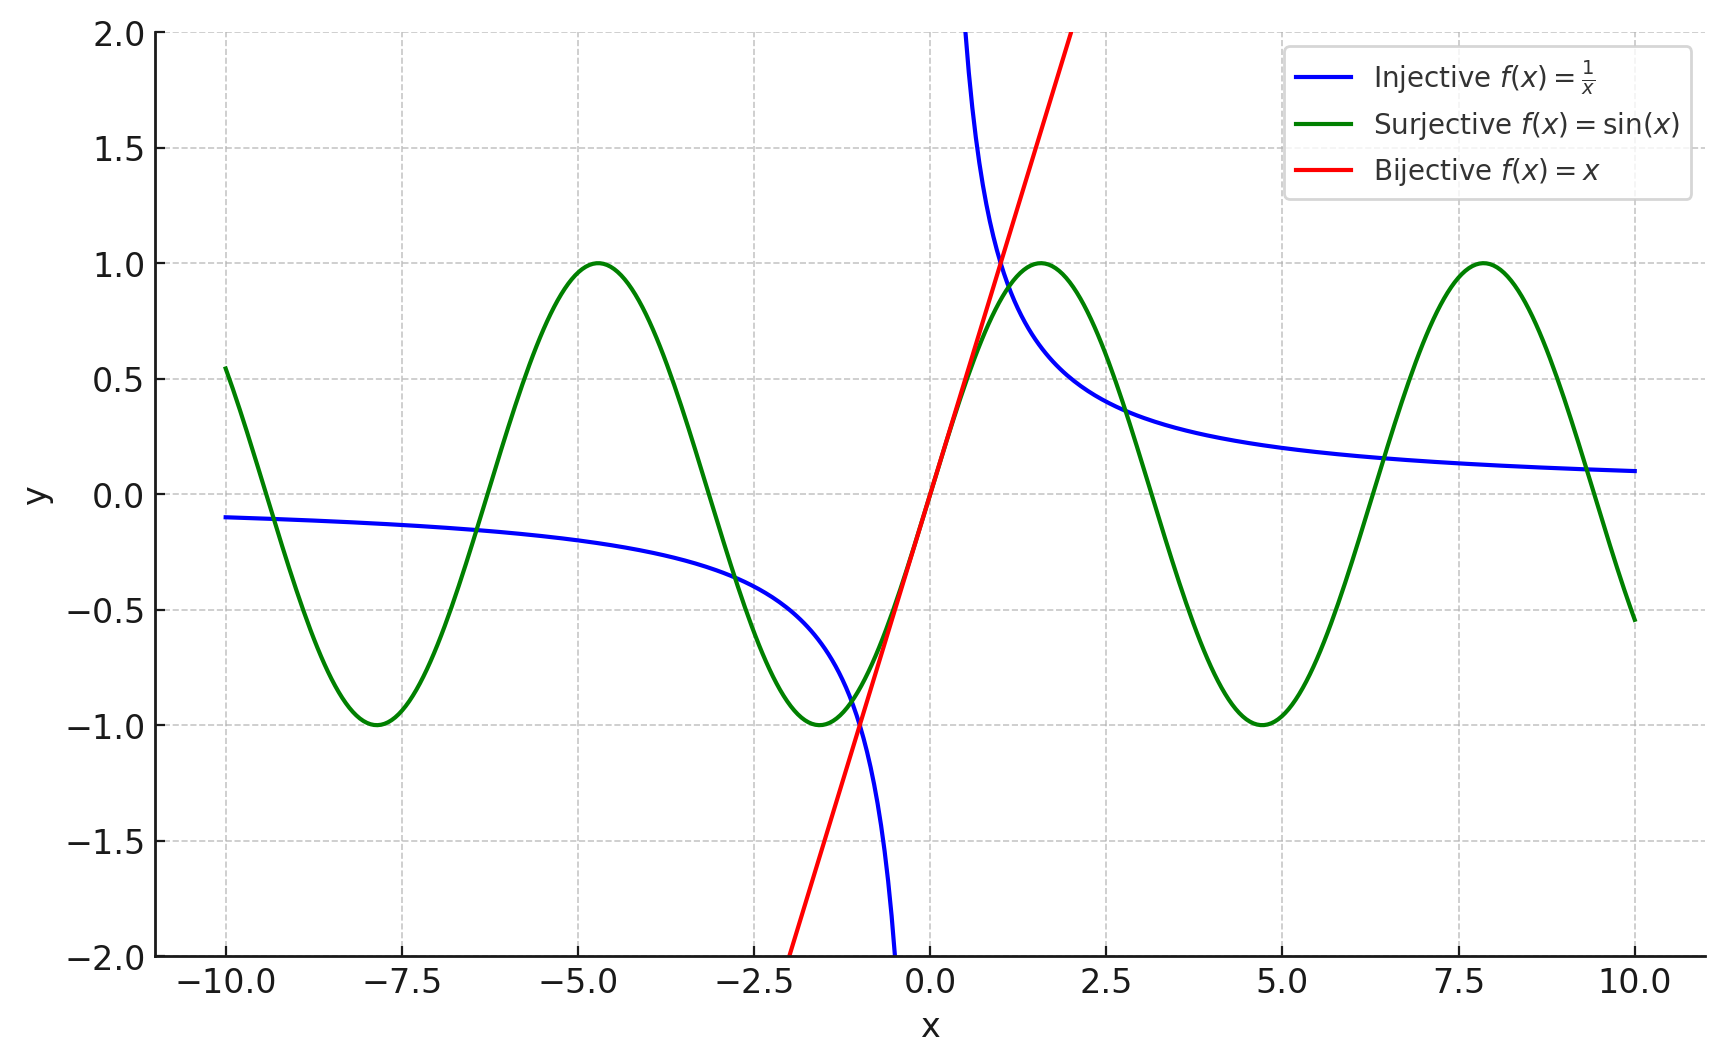
\includegraphics[width=0.75\linewidth]{Images/func.jpg}
    \caption{Examples of Special Mappings}
    \label{fig:fuc}
\end{figure}

Examine the figure \autoref{fig:fuc}, where one example of each type of function is shown. Fundamentally, when we define these functions, only two properties are involve:
\begin{itemize}
    \item A: It the mapping retrievable? (for every value in the image, we can find where it is from without any confusion.
    \item B: Is the mapping is full comparing to the preimage?(Whether every value in the preimage has a mapping to the image)
\end{itemize}
If A is satisfied, we call it injective function.

If B is satisfied, we call it surjective function.

If both A and B are satisfied, we say the function is bijective.

Using $A$, $B$, and $C$ to denote the set of injective, surjective, and bijective function respectively, it is therefore that :

    $$A\cap B = C$$

Which means that if a function is injective and surjective in the same time, it is bijective. 

And these will be all we need to know about function for now, since the rest of the properties will be discussed in single-variable calculus. This section aims only introduce the idea of injectivity, surjectivity, and bijectivity, 
%------------------------------------------------
\section{Summation}
Before we move on to the most important part of this chapter, sequence, we use this section to introduce a prerequisite for studying its properties. We introduce the Sigma sign.

In earlier chapters, we have seen exercises such as finding the expression of the sum of the first nth positive integer:
$$1 + 2 + \dots + (n-1) + (n)= \frac{n(n+1)}{2}$$ 
From now on, we will use the sigma notation to deal with the summation of numbers. Such as:
\subsection{Sigma Notation}
\begin{notation}[Sigma Notation]
    \[
\sum_{i=1}^{n} i = \frac{n(n + 1)}{2}
    \]
\end{notation}
Where $i$ is quite similar to iterator, or sometimes we also call counter in programming languages, and $n$ refers to the condition of termination. The expression right after the sigma sign is called \textbf{summand}.

Actually, this is not the only way to express summation, it is also equivalent to:
\[\sum_{1\leq i\leq n} i = \frac{n(n+1)}{2}\]

Also, like what we do for set, we can also write sigma notation using description, such as: 
\[
\sum_{1 \leq k \leq 100} k^2
\]

\( k \) is odd

\subsection{Properties and Techniques of Sigma Notation}
This part of the section shows how we can handle summation expressions.
One of the greatest convenience of sigma notation is that every expression is adjustable, we can change the variable as what we prefer as in the following example.
\begin{example} \label{exp:siginvariance}
 \[
\sum_{1 \leq k \leq n} a_k = \sum_{1 \leq k+1 \leq n} a_{k+1}
\]
\end{example}
This technique has a significant effect to some mathematical proofs.
Another points to keep in mind is that: always make the expression simple in terms of upper and lower boundary.
\begin{example}
    Examine this expression: 
    \[\sum_{k=0}^{n} k(k-1)(k-n)\]
    The sum when k equals to 0, 1, and $n$ is 0. In this case we cannot say it is a good expression, as what we want is the sum it self, while 0 does not matter for us. Therefore, we just fine-tune it to:
    \[\sum_{k=2}^{n-1} k(k-1)(k-n)\]
    This makes it concise and clear.
\end{example}

\subsubsection{Manipulation of Sigma Notation}
For a set \( K \), the following summation properties hold. Let \( c \) be a constant, and \( a_k \), \( b_k \) be sequences indexed by \( K \):

\begin{equation}
    \sum_{k \in K} c a_k = c \sum_{k \in K} a_k \quad \text{(Distributive Law)}
    \label{eq:constant_factor}
\end{equation}

\begin{equation}
    \sum_{k \in K} (a_k + b_k) = \sum_{k \in K} a_k + \sum_{k \in K} b_k \quad \text{(Associative Law)}
    \label{eq:summation_of_sums}
\end{equation}

\begin{equation}
    \sum_{k \in K} a_k = \sum_{p(k) \in K} a_{p(k)} \quad \text{(Commutative Law, as in example \autoref{exp:siginvariance})} 
    \label{eq:permutation_invariance}
\end{equation}
The proof is attached below.

\textbf{Proof of Constant Factor Law:}

Let \( c \) be a constant and \( a_k \) be a sequence indexed by a finite set \( K \). We want to show that \( \sum_{k \in K} c a_k = c \sum_{k \in K} a_k \).

By the definition of summation and the distributive property of multiplication over addition, we have:
\begin{equation}
    \sum_{k \in K} c a_k = c a_1 + c a_2 + \ldots + c a_n = c (a_1 + a_2 + \ldots + a_n) = c \sum_{k \in K} a_k.
\end{equation}
This concludes the proof of the constant factor law.

\textbf{Proof of Summation of Sums Law:}

Let \( a_k \) and \( b_k \) be sequences indexed by a finite set \( K \). We want to show that \( \sum_{k \in K} (a_k + b_k) = \sum_{k \in K} a_k + \sum_{k \in K} b_k \).

By the definition of summation and the associative and commutative properties of addition, we have:
\begin{equation}
    \begin{split}
\sum_{k \in K} (a_k + b_k) &= (a_1 + b_1) + (a_2 + b_2) + \ldots + (a_n + b_n) \\
&= (a_1 + a_2 + \ldots + a_n) + (b_1 + b_2 + \ldots + b_n) \\
&= \sum_{k \in K} a_k + \sum_{k \in K} b_k
\end{split}
\label{eq:sum_of_sums}
\end{equation}
This concludes the proof of the summation of sums law.

\textbf{Proof of Permutation Invariance Law:}

Let \( a_k \) be a sequence indexed by a finite set \( K \). Let \( p: K \to K \) be a bijection, which means \( p \) permutes the indices. We want to show that \( \sum_{k \in K} a_k = \sum_{p(k) \in K} a_{p(k)} \).

By the definition of summation and the fact that addition is commutative (the order does not matter), we have:
\begin{equation}
    \sum_{k \in K} a_k = a_1 + a_2 + \ldots + a_n = a_{p(1)} + a_{p(2)} + \ldots + a_{p(n)} = \sum_{p(k) \in K} a_{p(k)}.
\end{equation}
This concludes the proof of the permutation invariance law.
\subsubsection{Multiple Sums}
Sometimes we use sigma notation with multiple variables, just like what we can do to write loops in programming languages.

    
$$\sum_{1 \leq j, k \leq 3} a_j b_k = a_1b_1 + a_1b_2 + a_1b_3 + a_2b_1 + a_2b_2 + a_2b_3 + a_3b_1 + a_3b_2 + a_3b_3 $$


In the context of summation, we often encounter a situation where a sum is taken over a set of pairs. Specifically, let \( P(j, k) \) be a property involving the indices \( j \) and \( k \), and \( a_{j,k} \) be elements corresponding to these indices. The summation over all pairs \( (j, k) \) satisfying property \( P \) is equivalent to summing over all indices separately:

\[
\sum_{P(j,k)} a_{j,k} = \sum_{j,k} a_{j,k} \cdot P(j,k).
\]

This notation serves as a shorthand for expressing the sum over a subset of indices determined by the property \( P \).
There are also cases where we must use two sigma notation in the same time.

 
\begin{example}[Double Summation]
    When considering a double sum over a set of pairs, we often come across the following identity:

\begin{equation}
\sum_{j}\sum_{k} a_{j,k} [P(j,k)]
\end{equation}

where \( [P(j,k)] \) is an Iverson bracket which equals 1 if the property \( P \) holds for the pair \( (j,k) \) and 0 otherwise.
\end{example}


By interchanging the order of summation, we observe that:

\begin{equation}
\sum_{j}\sum_{k} a_{j,k} [P(j,k)] = \sum_{k}\sum_{j} a_{j,k} [P(j,k)].
\end{equation}

This property allows us to switch the order of summation without changing the result, which can be particularly useful in various mathematical analyses.

Double summation could also be used to simplify a given summation.
Considering the expression at the beginning of this section:
$$\sum_{1 \leq j, k \leq 3} a_j b_k = a_1b_1 + a_1b_2 + a_1b_3 + a_2b_1 + a_2b_2 + a_2b_3 + a_3b_1 + a_3b_2 + a_3b_3 $$

\begin{example}[Converting to Double Summation]
    \[
\sum_{1 \leq i,j,k \leq 3} a_j b_k = \sum_{\substack{i,j,k \\ 1 \leq i,j,k \leq 3}} a_j b_k \left[1 \leq j \leq 3\right] \left[1 \leq k \leq 3\right]
\]
\[
= \sum_j \sum_k a_j b_k \left[1 \leq j \leq 3\right] \left[1 \leq k \leq 3\right]
\]
\[
= \sum_j a_j \left[1 \leq j \leq 3\right] \sum_k b_k \left[1 \leq k \leq 3\right]
\]
\[
= \sum_j a_j \left[1 \leq j \leq 3\right] \left( \sum_k b_k \left[1 \leq k \leq 3\right] \right)
\]
\[
= \left( \sum_j a_j \left[1 \leq j \leq 3\right] \right) \left( \sum_k b_k \left[1 \leq k \leq 3\right] \right)
\]
\[
= \left( \sum_{j=1}^3 a_j \right) \left( \sum_{k=1}^3 b_k \right).
    \]

\end{example}
To explicit:
In the situation where we perform the same range of summation over each variable, the first two lines' triple summation is:
\[
(a_1b_1 + a_1b_2 + a_1b_3) + (a_2b_1 + a_2b_2 + a_2b_3) + (a_3b_1 + a_3b_2 + a_3b_3).
\]
Utilizing the distributive property to combine the summation operations into one involving \( a \), since \( a \) and each \( k \) for \( 1 \leq j \leq 3 \) are independent, yields (as in the third line):
\[
a_1(b_1 + b_2 + b_3) + a_2(b_1 + b_2 + b_3) + a_3(b_1 + b_2 + b_3).
\]

Consider a double sum over two independent indices, if the indices are independent, the summation of the product can be split into the product of two summations. For instance, the sum of products of \(a_j\) and \(b_k\) over \(j\) in \(J\) and \(k\) in \(K\) can be expressed as: \( (a_1 + a_2 + a_3)(b_1 + b_2 + b_3) \). This can be generalized to an expression:

\begin{equation}
\sum_{j \in J} \sum_{k \in K} a_j b_k = \left( \sum_{j \in J} a_j \right) \left( \sum_{k \in K} b_k \right),
\end{equation}
which is known as the \textbf{general distributive law}.
\begin{remark}
    If you are an agile reader, you must have noticed that this expression is a kind of representation of Cartesian sets in algebra. The general distributive law allows the sum over a function of elements from the Cartesian product of two sets to be expressed as the product of sums over each set if the function is separable into independent factors.
\end{remark}
\subsection{Exercises}
\begin{exercise}
    Express the triple sum
\[
\sum_{1 \leq i < j < k \leq 4} a_{ijk}
\]
as a three-fold summation (with three \(\sum\)'s), 

\begin{enumerate}[label=\alph*.]
    \item summing first on \( k \), then \( j \), then \( i \);
    \item summing first on \( i \), then \( j \), then \( k \).
\end{enumerate}
Also write your triple sums out in full without the \(\sum\)-notation, using parentheses to show what is being added together first.
\end{exercise}
\textbf{Solution:}

\textbf{(a)} \[
\sum_{i=1}^{4} \sum_{j=i+1}^{4} \sum_{k=j+1}^{4} a_{ijk} = 
\sum_{i=1}^{2} \sum_{j=i+1}^{3} \sum_{k=j+1}^{4} a_{ijk} = 
((a_{123} + a_{124}) + a_{134}) + a_{234}.
\]

\textbf{(b)} \[
\sum_{k=1}^{4} \sum_{j=1}^{k-1} \sum_{i=1}^{j-1} a_{ijk} = 
\sum_{k=3}^{4} \sum_{j=2}^{k-1} \sum_{i=1}^{j-1} a_{ijk} = 
a_{123} + (a_{124} + a_{134} + a_{234}).
\]

\begin{exercise}
    Demonstrate your understanding of \(\Sigma\)-notation by writing out the sums
\[
\sum_{k=0}^{5} a_k \quad \text{and} \quad \sum_{0\leq k^2 \leq 5} a_{k^2}
\]
in full. (Watch out—the second sum is a bit tricky.)

\end{exercise}
\textbf{Solution:}

The first sum is:
\[
a_0 + a_1 + a_2 + a_3 + a_4 + a_5
\]

The second sum, being tricky, $k \in \{-2, -1, 0, 1, 2\}$, therefore:
\[
a_4 + a_1 + a_0 + a_1 + a_4
\]

\begin{exercise}
    The general rule for summation by parts is equivalent to
\[
\sum_{0 \leq k < n} (a_{k+1} - a_k)b_k = a_nb_n - a_0b_0 - \sum_{0 \leq k < n} a_{k+1}(b_{k+1} - b_k), \quad \text{for } n \geq 0.
\]

Prove this formula by using the distributive, associative, and commutative laws.
\end{exercise}
Hint: Use Associative Law to LHS, try to make the indices of the two sums as similar as possible.
\begin{proof}
    \begin{align*}
        \text{LHS} &= \sum_{0\leq k < n} a_k b_{k+1} - \sum_{0\leq k < n} a_k b_k \\
        &= \sum_{0\leq k < n} a_k b_{k+1} - \sum_{-1\leq k < n-1} a_{k+1} b_{k+1} \\
        &= \sum_{0\leq k < n} a_k b_{k+1} - \sum_{0\leq k < n-1} a_{k+1} b_{k+1} \\
        &= \sum_{k=0}^{n-1} a_k b_{k+1} - \sum_{k=0}^{n-2} a_{k+1} b_{k+1} \\
        &= a_n b_{n-1} - a_0 b_0 + \sum_{k=0}^{n-2} a_k b_k - \sum_{k=0}^{n-2} a_{k+1} b_{k+1} \\
        &= a_n b_{n-1} - a_0 b_0 + \sum_{0\leq k < n-1} a_k (b_k - b_{k+1}) \\
        &= a_n (b_n - b_{n-1}) + a_n b_{n-1} - a_0 b_0 - \sum_{0\leq k < n-1} a_{k+1} (b_{k+1} - b_k) \\
        &= a_n (b_n - b_{n-1} + b_{n-1}) - a_0 b_0 - \sum_{0\leq k < n} a_{k+1} (b_{k+1} - b_k) \\
        &= a_n b_n - a_0 b_0 - \sum_{0\leq k < n} a_{k+1} (b_{k+1} - b_k) \\
        &= \text{RHS}
        \end{align*}
\end{proof}
\begin{exercise}
    Is the following expression correct or not? Give your reason.
    \[
\left( \sum_{i=1}^{n} a_i \right) \left( \sum_{j=1}^{n} \frac{1}{a_j} \right) = \sum_{1 \leq i \leq n} \sum_{1 \leq j \leq n} \frac{a_i}{a_j} = \sum_{1 \leq i \leq n} \sum_{1 \leq i \leq n} \frac{a_i}{a_i} = \sum_{i=1}^{n} 1 = n
\]
\end{exercise}
Consider the expression given by:
\[
\left( \sum_{i=1}^{n} a_i \right) \left( \sum_{j=1}^{n} \frac{1}{a_j} \right)
\]
and its expansion into a double sum:
\[
\sum_{1 \leq i \leq n} \sum_{1 \leq j \leq n} \frac{a_i}{a_j}
\]

It is claimed that this is equal to:
\[
\sum_{1 \leq i \leq n} \sum_{1 \leq i \leq n} \frac{a_i}{a_i} = \sum_{i=1}^{n} 1 = n
\]

However, this claim overlooks the fact that the double sum includes terms where \( i \neq j \), which are not necessarily equal to 1. Only when \( i = j \) does the term \( \frac{a_i}{a_j} \) simplify to 1, contributing to the count of \( n \).

Hence, the proper expansion of the double sum should be written as:
\[
\sum_{i=1}^{n} \sum_{j=1}^{n} \frac{a_i}{a_j} = \sum_{i=1}^{n} 1 + \sum_{\substack{i,j=1 \\ i \neq j}}^{n} \frac{a_i}{a_j}
\]
where the first sum on the right-hand side counts the \( n \) instances where \( i = j \), and the second sum accounts for the \( n(n-1) \) instances where \( i \neq j \).

The claim would only be true if all \( a_i \) are equal, which is a special case, not the general case. In the general case, the expression evaluates to something different than \( n \) due to the presence of terms where \( i \neq j \). 

Therefore, the original statement is incorrect unless the condition that all \( a_i \) are equal is specified.
%------------------------------------------------

\section{Sequence}
If everything so far is not a problem for you, congratulations, because you have known everything you need to know sequence. Sequence is an important concept that will be used throughout your journey of learning math. A Sequence
is defined as:
\begin{definition}
    A sequence is a function \( f: \mathbb{N} \to \mathbb{R} \), where \(\mathbb{N}\) is the set of natural numbers and \(\mathbb{R}\) is the set of real numbers. The value \( f(n) \) 
    is the \( n \)-th term of the sequence, often denoted as \( a_n \). Therefore, a sequence can be represented as \( \{a_n\}_{n=1}^{\infty} \) for an infinite sequence or \( \{a_n\}_{n=1}^{N} \) for a finite sequence of length \( N \).
\end{definition} 

\subsection{Introduction}
Sequences could be either infinite or finite. A \textit{sequence} is defined to be a function \( S \) whose domain \( D \) is a nonempty interval of integers. \( S \) is an \textit{infinite sequence} if \( D \) has the form \( \{a..\} \). % Usually \( a \) is 1 or 0.

\( S \) is a \textit{finite sequence} if \( D \) has the form \( \{a..b\} \) where \( a \leq b \). When \( |D| = n \), we will say that \( S \) is an \( n\text{-sequence} \). We will take the domain of an \( n\text{-sequence} \) to be the set \( \{1..n\} \). % But \( a \) could be 0, and then \( D \) is \( \{0..(n - 1)\} \).

The (natural) ordering of the domain of a sequence \( S \) gives a natural ordering to the ordered pairs in the set \( S \). If \( S \) is a 5-sequence, then
\[ S = \{(1, S(1)), (2, S(2)), (3, S(3)), (4, S(4)), (5, S(5))\} \]

\begin{example}
    Suppose \( D = \{1..10\} \), and we define the function \( S \) on \( D \) by

\[ S(i) = \text{the smallest prime factor of the integer } (1 + i). \]

Then \( D \) is a finite interval of integers, and so \( S \) is the sequence denoted by

\[ S = (2, 3, 2, 5, 2, 7, 2, 3, 2, 11). \]
\end{example}

\begin{definition}[Sum of Sequence]
    If \( S = (S_1, S_2, S_3, \ldots, S_n) \) is a finite sequence of numbers, the corresponding \textit{series} is the sum of the entries in \( S \)
    is:

\[ S_1 + S_2 + S_3 + \ldots + S_n. \]
\end{definition}
\subsection{Special Sequences}
This section introduces common sequences as well as their properties.
\subsubsection{Algorithmic Sequence}
Algorithmic sequences are a fundamental concept in both computer science and mathematics, forming the backbone of algorithm design and analysis. These sequences are typically defined as an ordered set of steps or instructions, aimed at solving a specific problem or accomplishing a particular computation.
\begin{definition}[Arithmetic Sequence]
    An arithmetic sequence of the form
\[
a, a + d, a + 2d, \ldots, a + nd, \ldots
\]
where the initial term \( a \) and the common difference \( d \) are real numbers.
\end{definition}
Usually, the notation $a_n$ is used to express the nth term of a sequence (starting from 0). For the example in the 
definition, we have $a_0 = a$ and $a_n = a_0 + nd$. 
We also have:
$$a_1 = a_0 + d$$
$$a_2 = a_1 + d$$
$$\dots$$
$$a_n = a_0 + nd$$ 
for $n>=1$, $n\in \mathbb{Z}$:
$$a_n = a_{n-1} + d$$
These formula shows the linking between consecutive terms in an arithmetic sequence. We know that the sum
$s$ of the sequence is:
\begin{align*}
    S & =\ a_{0} \ +\ a_1\ \ +\ \dotsc \ +\ a\_n\\
    S & =\ a_{0} \ +\ a_{0} +d\ +\ \dotsc \ +\ a_{n-1} +d
    \end{align*}
The sum is expressed in infinite terms, and it is called \textbf{open form equation}. Accordingly, there are also \textbf{closed form
equations}.
\begin{definition}[Open Form]
    An \textit{open form} or \textit{non-closed form} expression, on the other hand, does not have a finite standard representation and often requires recursive or iterative methods for evaluation. It may involve summations, integrals, or other operations that are not easily simplified into a finite number of operations.
\end{definition}
\begin{definition}[Closed Form]
    A \textit{closed form} expression is a mathematical expression that can be evaluated in a finite number of standard operations. It typically involves constants, variables, and operations from algebra, calculus, and other areas of mathematics that can be computed in a finite number of steps.
    A closed form expression provides a direct way to compute the term of a sequence without the need for recursion.
\end{definition}

Is the open form good for calculating the sum of a sequence? Suppose now I want to know $S_{100}$ (The sum of the first 100th terms),
with the open form, I still have to calculate 99 terms using the definition of this sequence. So is there a way 
to make it possible that we get the sum in one step? Think about closed form. The closed form allows us to calculate
the sum directly. But is it possible to transform an open expression to closed form? If possible, how?

You may already notice that the open form has a property of infinity, and each step is somewhat related.
Isn't it a perfect problem to be solved by mathematical induction? We will leave this proof as a exercise, and here we provide another direct proof
by the symmetry of arithmetic sequence.
\begin{theorem}[Sum of Arithmetic Sequence]
    For  arithmetic sequence \( a_0, a_1, \ldots, a_{n-1} \), where each term can be expressed as \( a_i = a_0 + id \) and \( d \) is the common difference. The sum of the first nth terms is:
    \[ S = \frac{n}{2}[2a_0 + (n-1)d] \] or \[ S = \frac{n}{2}(a_0 + a_{n-1}) \] where \[ a_n = a_0 + nd \]
\end{theorem}
\begin{remark}
    We are trying to find the sum of the first n terms, and the first term is $a_0$, so the last term is
    $a_{n-1}$.
\end{remark}
\begin{proof}
    Consider an arithmetic sequence \( a_0, a_1, \ldots, a_n \), where each term can be expressed as \( a_i = a_0 + id \) and \( d \) is the common difference.
    \item Write the sum of the sequence in order:
\[
S = a_0 + (a_0 + d) + (a_0 + 2d) + \ldots + (a_0 + (n-1)d)
\]

\item Write the sum of the sequence in reverse order:
\[
S = (a_0 + (n-1)d) + (a_0 + (n-2)d) + \ldots + a_0
\]

\item Add these two equations together, every pair of terms within the brackets forms: \[ 2a_0 + (n-1)d \]

\item Since each term appears in a pair, there are \( n \) such pairs.

\item The resulting equation is \( 2S = n[2a_0 + (n-1)d] \).

\item Solving for \( S \) gives us \( S = \frac{n}{2}[2a_0 + (n-1)d] \) or \( S = \frac{n}{2}(a_0 + a_n) \), where \( a_n = a_0 + (n-1)d \).
\end{proof}


\subsubsection{Geometric Sequence}
Geometric sequence is the other important and common sequence that involved in problem-solving of computer
Science. 
A geometric sequence, also known as a geometric progression, is a sequence of numbers where each term after 
the first is found by multiplying the previous term by a fixed, non-zero number called the common ratio. 
Mathematically, a geometric sequence is defined as follows:
\begin{definition}[Geometric Sequence]
    Given the first term \( a_0 \) (also referred to as \( a_1 \) in some texts) and the common ratio \( r \), the \( n \)-th term of a geometric sequence \( a_n \) can be expressed as:
\[
a_n = a_0 \cdot r^n \quad \text{for } n \geq 0
\]
where \( n \) is a non-negative integer representing the position of the term in the sequence.
\end{definition}    

The common ratio \( r \) can be any real number. If \( |r| < 1 \), the terms of the sequence 
will get progressively smaller and approach zero. If \( |r| > 1 \), the terms will grow progressively 
larger. If \( r = 1 \), the sequence is constant, and if \( r = -1 \), the sequence will alternate 
between two values.

We can deduce the sum of a specific geometric sequence by direct proof.
\begin{theorem}[Sum of Geometric Sequence]
    
\end{theorem}

\begin{proof}
    Consider a geometric sequence with the first term \( a_0 \) and the common ratio \( r \) where \( r \neq 1 \). The sequence is given by:
\[ a_0, a_0r, a_0r^2, \ldots, a_0r^{n-1} \]

The sum of the first \( n \) terms of the sequence, denoted by \( S_n \), is:
\[ S_n = a_0 + a_0r + a_0r^2 + \ldots + a_0r^{n-1} \]

To find a formula for \( S_n \), multiply the entire sequence by \( r \):
\[ rS_n = a_0r + a_0r^2 + a_0r^3 + \ldots + a_0r^n \]

Subtract the original sum \( S_n \) from this new sum \( rS_n \) to get a telescoping series:
\[ rS_n - S_n = a_0r^n - a_0 \]

Solving for \( S_n \) gives us:
\[ S_n = \frac{a_0(1 - r^n)}{1 - r} = \]

This is the sum formula for the first \( n \) terms of a geometric sequence when \( r \neq 1 \). If \( r = 1 \), the sequence is constant, and the sum of the first \( n \) terms is simply \( n \) times the first term \( a_0 \).
\end{proof}
%----------------------------------------------------------------------
\subsubsection{characteristic Sequence}
\begin{definition}[Characteristic Sequence]
    Suppose that \( U \) is some given \( n \)-set whose elements have been \textit{indexed} (listed in a certain order) so that \( U = \{x_1, x_2, \ldots, x_n\} \). If \( A \) is a subset of \( U \), the \textit{characteristic sequence} of \( A \) is the function whose domain is \( \{1..n\} \) defined by

\[
X^A_i = X^A(i) = 
\begin{cases} 
1 & \text{if } x_i \in A \\
0 & \text{if } x_i \notin A 
\end{cases}
\]
\end{definition}

\begin{example}
    If \( U \) is the set of the first 10 odd positive integers, \( A \) is the subset of primes in \( U \), and \( B \) is the set of multiples of 3 in \( U \), then
    
    \[
    \begin{aligned}
    &U = \{1, 3, 5, 7, 9, 11, 13, 15, 17, 19\} &&// x_i = 2i - 1. \\
    &A = \{3, 5, 7, 11, 13, 17, 19\} \\
    &B = \{3, 9, 15\} \\
    &X^A = (0, 1, 1, 1, 0, 1, 1, 0, 1, 1) \\
    &X^B = (0, 1, 0, 0, 1, 0, 0, 1, 0, 0).
    \end{aligned}
    \]
    \end{example}

    Characteristic sequences may be used as an implementation model for subsets of any given indexed set \( U \). The set operations may be done on these sequences:
    \[
    X^{A \cap B}_i = X^A_i \times X^B_i;
    \]
    \[
    X^{A \cup B}_i = X^A_i + X^B_i - X^A_i \times X^B_i;
    \]
    \[
    X^{A \setminus B}_i = X^A_i - X^A_i \times X^B_i.
    \]
    
    If \( A \subseteq B \) then
    \[
    X^A_i \leq X^B_i \quad \text{for each index } i,
    \]
    and
    \[
    |A| = \sum_{i=1}^{n} X^A_i.
    \]

%----------------------------------------------------------------------
\subsection{Exercises}
\begin{exercise}
    Find the sum of arithmetic sequence using mathematical induction. Try \textbf{NOT} use the conclusion in this section.
\end{exercise}
Hint: Consider the sum of the first nth positive integer. Try to make assumption by taking it as an arithmetic sequence.
\begin{proof}
    Let \( S(n) \) denote the sum of the first \( n \) terms of an arithmetic sequence with the first term \( a_0 \) and common difference \( d \).
    \begin{itemize}
        \item \textbf{Base Case (\( n = 1 \))}: The sum of the sequence with only the first term is the first term itself, \( S(1) = a_0 \).
        \item \textbf{Inductive Step}: Assume that the sum of the first \( k \) terms \( S(k) \) is given by a certain formula. We want to show that the sum of the first \( k+1 \) terms \( S(k+1) \) can be expressed using the same formula.
        \end{itemize}
        
        For the base case, we can easily see that:
        \[
        S(1) = a_0
        \]
        As $\sum_{1}^{n}i = \frac{n(n+1)}{2}$, which could be taken as an arithmetic sequence with $a_0=1$ and
        $a_n=n$.
        By this, assume that the sum of the first \( k \) terms is:
        \[
        S(k) = \frac{k}{2} [a_0 + a_n]
        \]
        equivalent to
        \[
        S(k) = \frac{k}{2} [2a_0 + (k-1)d]
        \]
        
        To prove the inductive step for \( S(k+1) \), consider:
        \[
        S(k+1) = S(k) + a_0 + kd
        \]
        
        Substituting the inductive hypothesis into the above equation yields:
        \[
        S(k+1) = \frac{k}{2} [2a_0 + (k-1)d] + a_0 + kd
        \]
        
        After simplifying, we aim to show that:
        \[
        S(k+1) = \frac{k+1}{2} [2a_0 + kd]
        \]
        
        This will complete the proof if we can establish that the simplified version of \( S(k+1) \) matches the form of the inductive hypothesis.
\end{proof}
\begin{exercise}
    Prove the sum of geometric sequence  is \( S_n = \frac{a_0(1 - r^n)}{1 - r} = \) using mathematical induction.
\end{exercise}
\begin{proof}
    We want to prove that the sum of the first \( n \) terms of a geometric sequence \( S_n \) with the first term \( a \) and common ratio \( r \) (where \( r \neq 1 \)) is given by:

\[ S_n = \frac{a(1 - r^n)}{1 - r} \]

\textbf{Base Case (n=1):}

The sum of the first term is simply the term itself:

\[ S_1 = a \]

which agrees with the formula.

\textbf{Inductive Step:}

Assume the formula holds for \( n = k \), that is,

\[ S_k = \frac{a(1 - r^k)}{1 - r} \]

We need to prove that it also holds for \( n = k+1 \):

\[ S_{k+1} = \frac{a(1 - r^{k+1})}{1 - r} \]

Starting with the inductive hypothesis for \( S_k \) and adding the \( (k+1) \)-th term \( ar^k \) to both sides, we have:

\[ S_k + ar^k = \frac{a(1 - r^k)}{1 - r} + ar^k \]

Simplifying, we obtain:

\[ S_{k+1} = S_k + ar^k = \frac{a - ar^{k+1}}{1 - r} \]

which is the same as the formula for \( S_{k+1} \), thus completing the proof.
\end{proof}
\begin{exercise}
    Given a sequence \( \{a_n\} \) and a series \( S_n = an^2 + bn + c (a \neq 0) \).

\begin{enumerate}
    \item Find the general term \( a_n \);
    \item Is the sequence \( \{a_n\} \) an arithmetic sequence?
\end{enumerate}
\end{exercise}
Hint: How can we get the value of a term from the sum of a sequence?
\textbf{Solution:}

\begin{enumerate}
    \item For \( n \geq 2 \), \( a_n = S_n - S_{n-1} = (an^2 + bn + c) - [a(n-1)^2 + b(n-1) + c] \) \\
    \( = (b+a) + (n-1) \cdot 2a \),
    
    Therefore, for \( n=1 \), \( a_1 = (b+a) + (1-1) \cdot 2a = b + a + c - S_1 \), \\
    and the general term is
    \[
    a_n = 
    \begin{cases}
        a + b + c & (n=1) \\
        (b+a) + (n-1) \cdot 2a & (n \geq 2)
    \end{cases}
    \]

    \item Since \( c = 0 \), \( a_n \) can be simplified to \( a_n = a + b \), which is constant and equals \( 2a \) when \( n \geq 2 \). This implies \( \{a_n\} \) is an arithmetic sequence with common difference \( 2a \), provided \( a, b \) are constants and \( a \neq 0 \).
    
    Note: From \( S_n \) we can deduce \( a_n = S_n - S_{n-1} \) when \( n \geq 2 \). Since \( a_1 = S_1 \), the sequence \( a_n = S_n - S_{n-1} \) (for \( n \geq 2 \)) and \( a_1 \) is the first term. The sequence \( \{a_n\} \) is an arithmetic sequence.
    
    Therefore, the general term \( a_n \) can be expressed as:
    \[
    a_n = 
    \begin{cases}
        S_1 & (n=1) \\
        S_n - S_{n-1} & (n \geq 2)
    \end{cases}
    \]
    
    Given the series \( \{a_n\} \) with \( S_n = an^2 + bm + c (a \neq 0) \), the sequence \( \{a_n\} \) is an arithmetic sequence with common difference \( 2a \) when \( c = 0 \).
\end{enumerate}

\begin{exercise}
    Given constants $a$, $b$, $c$, consider the sum $S_n = 1^2 + 2^2 + 3^2 + \ldots + n(n+1)^2 = \frac{n(n+1)}{12}(an^2 + bn + c)$, where $an^2 + bn + c \neq 0$.
\end{exercise}
\begin{proof}
    For $n=1$, we have $\frac{1}{6}(a+b+c)$, thus $a_1 = 4 = \frac{1}{6}(a+b+c)$.
For $n=2$, we have $\frac{22}{2} = 11 = \frac{1}{2}(4a+b+c)$, thus $a_2 = 22 = 9a + 3b + c$.
For $n=3$, $a_3 = 70 = 9a + 3b + c$.\\

From these equations, we find that:
\begin{align*}
    a + b + c &= 24 \\
    4a + b + c &= 44 \\
    9a + 3b + c &= 70
\end{align*}

Solving the system, we get $a=3$, $b=11$, $c=10$.
For \(n = 1, 2, 3\), the sum can be expressed as:
\[
1 \cdot 2^2 + 2 \cdot 3^2 + \ldots + n(n+1)^2 = \frac{n(n+1)}{12}(3n^2 + 11n + 10),
\]
thus, \(S_n = 1 \cdot 2^2 + 2 \cdot 3^2 + \ldots + n(n+1)^2\).

For a general term \(k\), \(S_k = \frac{k(k+1)}{12}(3k^2 + 11k + 10)\). Therefore,
\[
S_{k+1} = S_k + (k+1)(k+2)^2
\]
\[
= \frac{k(k+1)}{12}(3k^2 + 11k + 10) + (k+1)(k+2)^2
\]
\[
= \frac{k(k+1)}{12}((k+2)(3k+5) + (k+1)(k+2)^2)
\]
\[
= \frac{(k+1)(k+2)}{12}(3k^2 + 5k + 12k + 24)
\]
\[
= \frac{(k+1)(k+2)}{12}(3(k+1)^2 + 11(k+1) + 10).
\]

Hence, by induction, we can show that for \(n = k+1\) the sum is valid.

Finally, with \(a = 3\), \(b = 11\), \(c = 10\), we confirm that the given sequence is indeed a second-order arithmetic sequence.
\end{proof}

\begin{exercise}
    Evaluate:
    \begin{enumerate}
        \item $S = \sum_{1}^{n} \frac{N}{2^n}$
        \\
        \item $S = \sum_{1}^{n} \frac{3n-2}{5^{n-1}}$  
    \end{enumerate}
\end{exercise}

\textbf{Solution:}

(1) Given the series \( S_n = \frac{1}{2} + \frac{2}{4} + \frac{3}{8} + \cdots + \frac{n}{2^n} \), we can write:

\[
S_n - \frac{1}{2}S_n = \frac{1}{2} + \frac{1}{4} + \frac{1}{8} + \cdots + \frac{1}{2^n} - \frac{n}{2^{n+1}}
\]

This simplifies to:

\[
\frac{1}{2}S_n = \frac{1}{2} \left(1 - \left(\frac{1}{2}\right)^n\right) = \frac{1}{2} - \frac{1}{2^{n+1}} = \frac{1}{2} - \frac{n}{2^{n+1}} + \frac{n}{2^{n+1}}
\]

Hence, the series sum is:

\[
S_n = 2 - \frac{1}{2^{n-1}} - \frac{n}{2^n} = 2 - \frac{n+2}{2^n}
\]

(2) Considering the series \( S_n = 1 + \frac{4}{5} + \frac{7}{25} + \cdots + \frac{3n-2}{5^{n-1}} \), we proceed similarly:

\[
\left(1 - \frac{1}{5}\right)S_n = 1 + \frac{3}{5} + \frac{3}{25} + \cdots + \frac{3}{5^{n-1}} - \frac{3n-2}{5^n}
\]

The terms form a geometric series, so we get:

\[
S_n = 1 + \frac{3}{5} \left(1 + \frac{1}{5} + \frac{1}{25} + \cdots + \frac{1}{5^{n-2}}\right) - \frac{3n-2}{5^n}
\]

Applying the formula for the sum of a geometric series, we find:

\[
S_n = 1 + \frac{3}{5} \left(\frac{1 - \left(\frac{1}{5}\right)^{n-1}}{1 - \frac{1}{5}}\right) - \frac{3n-2}{5^n}
\]

Simplifying, we obtain:

\[
S_n = 1 + \frac{3}{5} \left(\frac{5^n - 5}{4 \cdot 5^{n-1}}\right) - \frac{3n-2}{5^n}
\]

Further simplification gives us:

\[
S_n = \frac{35}{16} - \frac{12n+7}{16 \cdot 5^{n-1}}
\]
%------------------------------------------------

\chapterimage{chap2.png} % Chapter heading image
\chapterspaceabove{5.75cm} % Whitespace from the top of the page to the chapter title on chapter pages
\chapterspacebelow{10cm} % Amount of vertical whitespace from the top margin to the start of the text on chapter pages
\chapter{Algorithm and Number}

Computer Science is most commonly known as an engineering subject, while the unanimous pursuit of all engineering subjects are solving problems. This chapter delves in to methods to solve problems, which is also known as \textbf{algorithm}. In the world of Computer Science, everything is proceeded in a methodical manner, and the very dependency of this is algorithm. Meanwhile, we will introduce pseudocode, one of the most important tools for algorithm analysis, as well as the representation of number in Computer Science.

%------------------------------------------------

\section{Algorithm and Algorithm Analysis}
	This Section discusses what is algorithm, and more importantly, how algorithms
	are assessed.

    \subsection{Algorithm}
    \subsubsection{What is an Algorithm?}
    \begin{definition}[Algorithm] \label{def:algo}
        An algorithm is a well-defined, step-by-step procedure or sequence of instructions designed to solve a specific class of problems:
        \begin{itemize}
            \item Each step in an algorithm must be clear and unambiguous. 
            \item Algorithms must be solvable, meaning they should be able to produce a correct solution for any valid input within a finite amount of time.
            \item An algorithm must terminate, i.e., it should have a defined end, at which point the goal has been achieved and the final output is produced.
        \end{itemize} 
    \end{definition}
    Here is an example of multiplication algorithm for better understanding of the concept.
    \begin{example}[Russian Peasant Multiplication]
        To find the product of integers \( M \) and \( N \), both larger than one:

        \begin{enumerate}
            \item Start two columns on a page, one labeled ``A'' and the other ``B''; and put the value of \( M \) under A and the value of \( N \) under B.
            
            \item Repeat
            \begin{itemize}
                \item[(a)] calculate a new A-value by multiplying the old A-value by 2; and
                \item[(b)] calculate a new B-value by dividing the old B-value by 2 and reducing the result by a half if necessary to obtain an integer;
            \end{itemize}
            Until the B-value equals one.
            
            \item Go down the columns crossing out the A-value whenever the B-value is even.
            
            \item Add up the remaining A-values and ``return'' the sum.
        \end{enumerate}
    \end{example}
    To show how it works, assume $A=73$ and $B=41$.

\begin{table}[H]
\centering
\begin{tabular}{c|c}
\hline
A & B \\
\hline
73 & 41 \\
146 & 20 (20\(\frac{1}{2}\) is reduced to 20) \\
292 & 10 \\
584 & 5 \\
1168 & 2 (2\(\frac{1}{2}\) is reduced to 2) \\
2336 & 1 \\
\hline
\end{tabular}
\caption{Execution of RPM}
\end{table}

Sum of the remaining A-values: $2336+584+73=2993$.

Let's review this algorithm referring to definition \autoref{def:algo}. 
\begin{enumerate}
    \item Clarity and Accuracy: All the instructions are clear and manipulable, nothing is ambiguous.
    
    \item Solvability: It is no doubt that for any two real numbers, we can find their product.
    
    \item Termination: For which ever numbers, we can always solve the problem in limited steps, as the terminate condition is when $B=1$, while B is divided by 2 (integer division) repetitively. 
\end{enumerate}

Hence, the RPM is a good example of algorithm, and with this, we could tell whether
something else is an algorithm or not.
\subsubsection{Pseudocode}
Pseudocode is a simplified, half-code, half-natural language script used by software developers and algorithm designers to outline the structure of a program or algorithm. It's not executable code, but rather a high-level representation of the algorithm's logic. The purpose of pseudo-code is to express the design of an algorithm in a form that can be easily translated into actual programming languages. It is written in a way that is understandable to people who do not necessarily know the syntax of programming languages. Pseudo-code allows the designer to focus on the core logic of the algorithm without getting bogged down with the syntactic details of a particular programming language. It often uses control structures like if-then-else, while, for, and others that are common to many high-level languages.
Here's the RPM transcribed in pseudocode:
\begin{algorithm}[H]
	\caption{Russian Peasant Multiplication}\label{alg:rpm}
	\begin{algorithmic}[1]
	\Procedure{RPM}{$A, B$}
		\State $product \gets 0$
		\While{$B > 0$}
			\If{$B$ is odd}
				\State $product \gets product + A$
			\EndIf
			\State $A \gets A \times 2$
			\State $B \gets B \div 2$
		\EndWhile
		\State \textbf{return} $product$
	\EndProcedure
	\end{algorithmic}
	\end{algorithm}
	
	All later algorithm in this book will be presented using pseudocode.
%------------------------------------------------

\subsection{Algorithm Analysis}

\par Now let's take a look at this algorithm from another aspects. Is this a good or a bad algorithm. People assess algorithms by examine its \textbf{complexity}, which could be either \textbf{space complexity} or \textbf{time complexity}. The former refers to the the relationship between the input and the space needed to execute the algorithm, the latter, similarly, refers to the time needed. Many tools are available to quantify complexity, for both space and time complexity, \textbf{the big O notation} is the most common measurement. 
\begin{definition}[The Big O Notation]\label{Big O}
    Big O notation is used to classify algorithms according to how their running time or space requirements grow as the input size grows. The notation describes an upper limit on the time an algorithm could possibly take to complete, given the size of the input. For a function \( f(n) \), where n is the scale of input for the algorithm, the Big O notation is formally defined as follows with $c$ as a positive constant:
    $$O(f(n)) = \{ g(n) : \text{Where } c \text{ and } n_0 
	\text{ such that } 0 \leq g(n) \leq c \cdot f(n) \text{ for all } n \geq n_0 \}$$
\end{definition}

The following table provides common time complexities using Big O notation:

\begin{table}[ht]
\centering
\begin{tabular}{@{}cc@{}}
\toprule
\( f(n) \) & Description \\ \midrule
1 & Constant \\
\( \log n \) & Logarithmic \\
n & Linear \\
\( n \log n \) & Linearithmic \\
\( n^2 \) & Quadratic \\
\( n^3 \) & Cubic \\
\( 2^n \) & Exponential \\ 
\(n!\) & Factorial \\
\bottomrule
\end{tabular}
\caption{Common time complexities in Big O notation}
\end{table}
We can visualize it using function graph
\begin{figure}[H]
    \centering
    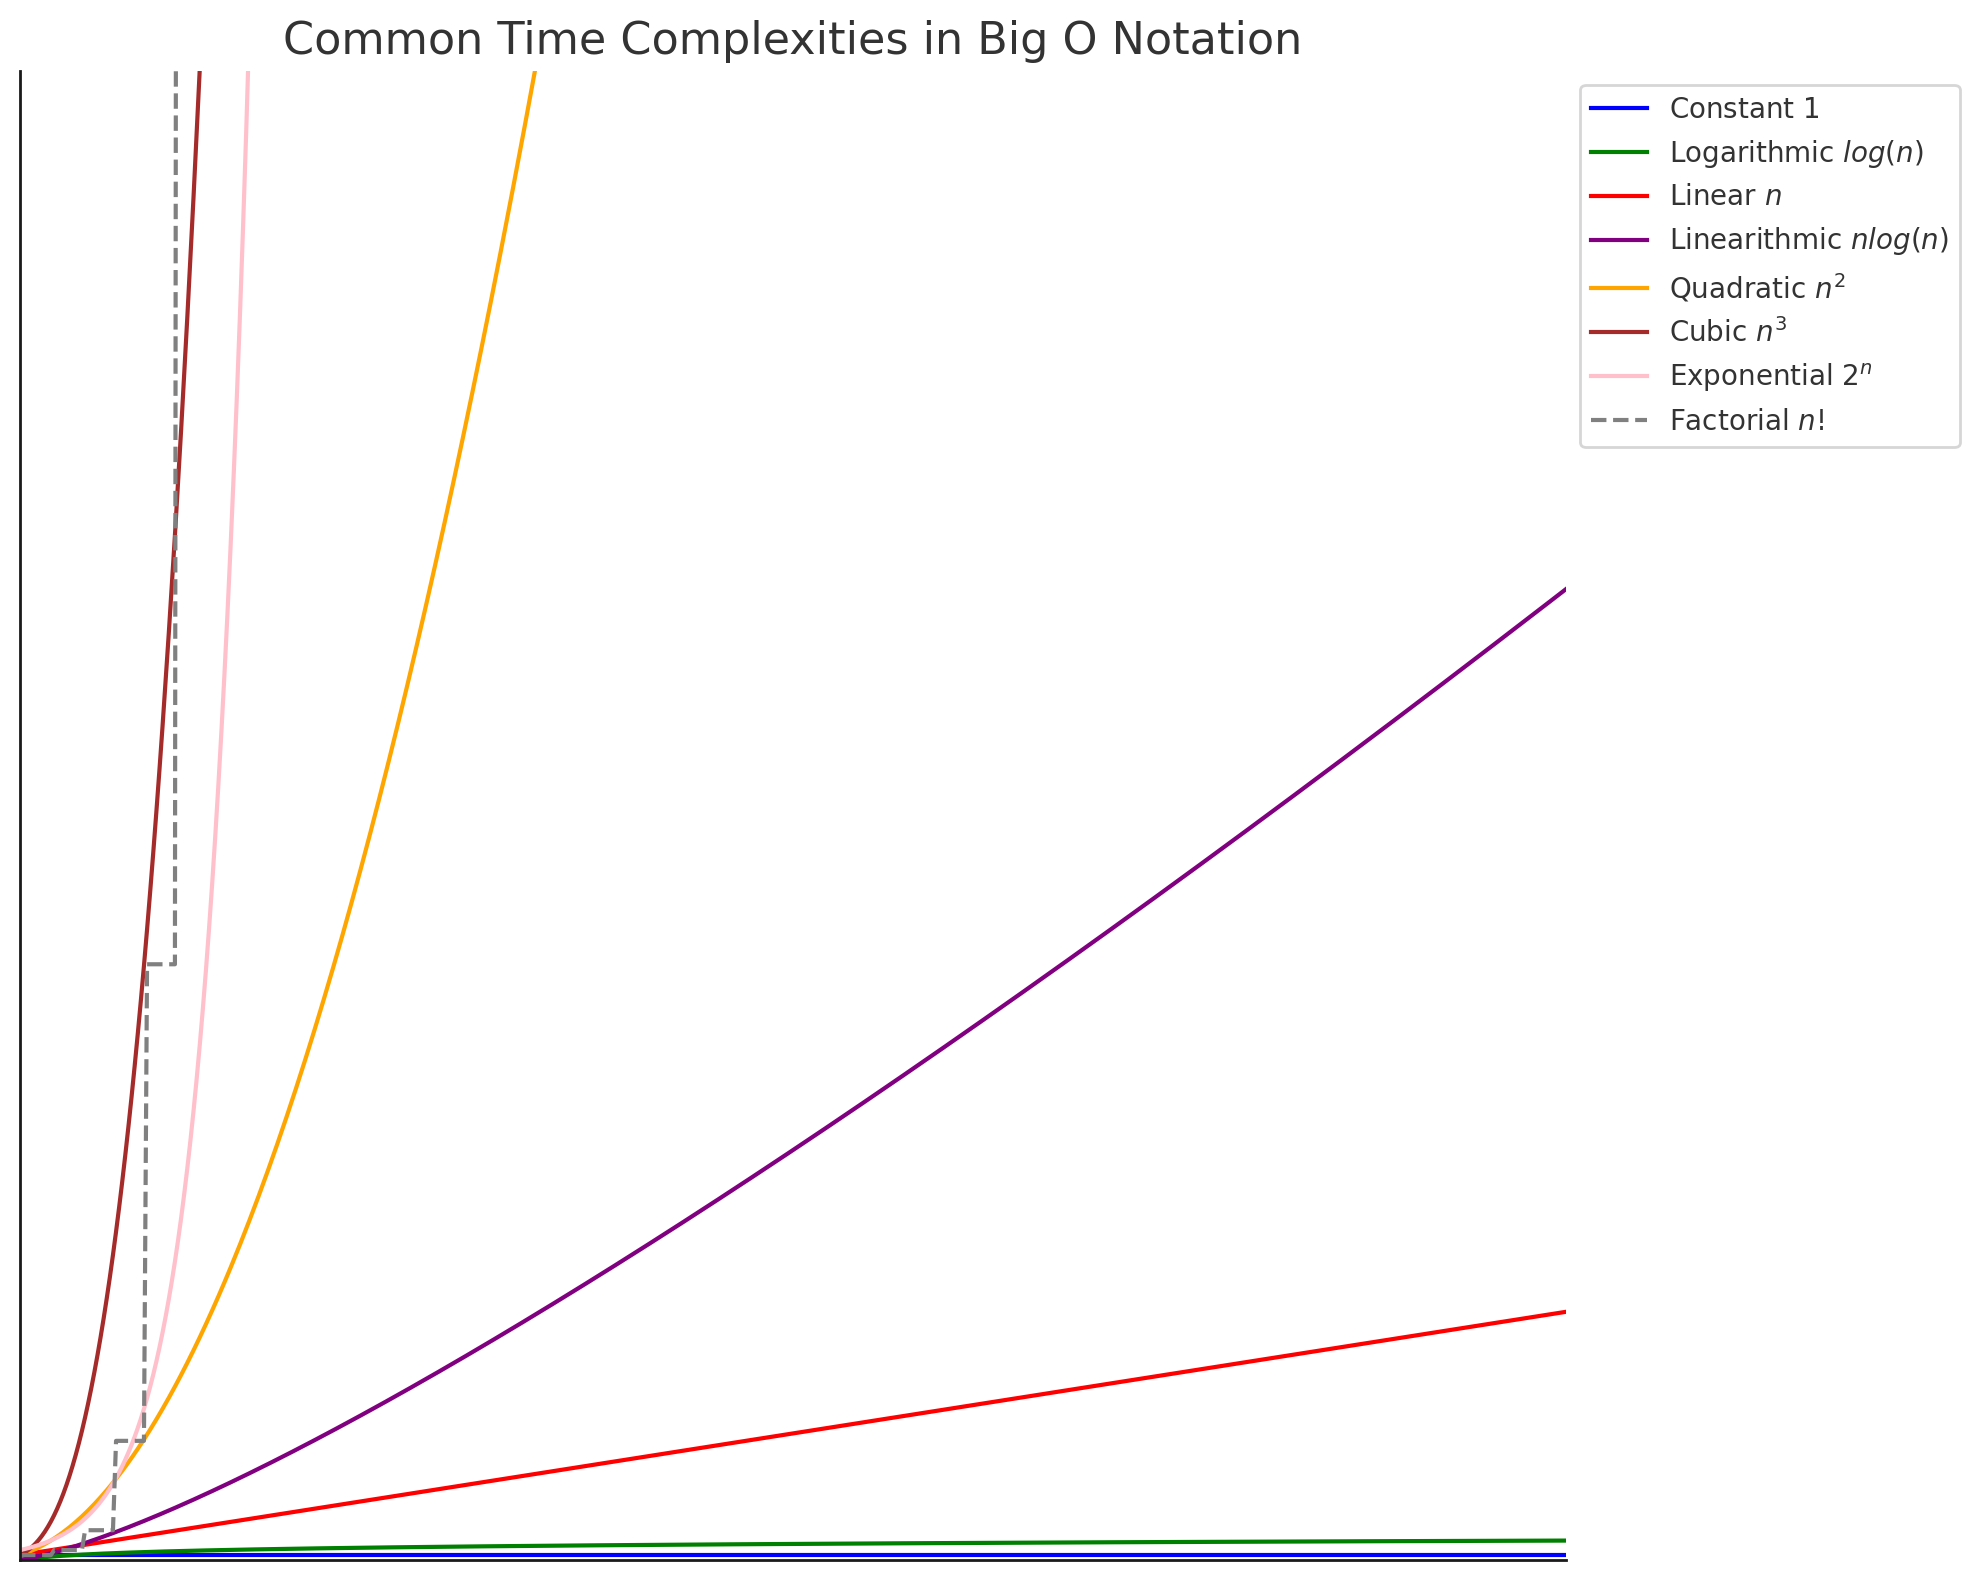
\includegraphics[width=0.8\linewidth]{Images/time complexity.png}
    \caption{Time Complexity Visualization}
    
\end{figure}
So which space and time complexity does this algorithm fall in? 
\subsubsection{Time Complexity}
To analyze the time complexity, we usually focus on the termination condition or the number of iteration for the algorithm. For the real number $B$ in RPM, each time it is divided by 2 until $B = 1$. Therefore, the total number of iteration will be $\log_2 B$, which is categorized in \( O(\log n) \).
\begin{remark}
    Actually, the time complexity of an algorithm could be shown by strict proof using MI. Here is the proof on the time complexity of RPM.
    \begin{proof}
        We will use mathematical induction to prove that the number of steps in the algorithm is proportional to \( \log_2(B) \).

\noindent \textbf{Base Case:}\\
When \( B = 1 \), the algorithm requires only one step. This is consistent with \( \log_2(1) = 0 \), which satisfies our complexity class \( O(\log n) \).

\noindent \textbf{Inductive Hypothesis:}\\
Assume that for a positive integer \( k \), when \( B = k \), the algorithm operates within \( \log_2(k) \) steps.

\noindent \textbf{Inductive Step:}\\
Consider \( B = 2k \). In the first step of the algorithm, \( B \) is halved to \( k \), and \( S \) is doubled. From this point, based on our inductive hypothesis, reaching \( B = 1 \) requires \( \log_2(k) \) steps.

Hence, for \( A = 2k \), the total number of steps is \( \log_2(k) + 1 \). Using the properties of logarithms, we have:
\begin{align*}
\log_2(k) + 1 &= \log_2(k) + \log_2(2) \\
&= \log_2(2k)
\end{align*}

Therefore, for any \( A = 2k \), the total number of steps is also \( \log_2(2k) \), proving that for any positive integer \( A \), the time complexity of the Russian Peasant Multiplication is \( O(\log A) \).
    \end{proof}
\end{remark}
%------------------------------------------------
\subsubsection{Space Complexity}
The space complexity of the Russian Peasant Multiplication algorithm is determined by the amount of memory required to store the operands and the intermediate results. Initially, only two numbers need to be stored: the multiplicands. As the algorithm proceeds, we need additional space to keep track of the current product. Since the algorithm does not use any complex data structures and only requires a fixed number of variables, the space complexity is \( O(1) \), indicating constant space usage. It does not depend on the size of the input operands, as the memory required does not increase with larger numbers.
%------------------------------------------------
\subsection{Exercises}
\begin{exercise}
    A non-recursive Square and Multiply Algorithm to calculate \( b^n \).

\textbf{Precondition:} \( n \) is a positive integer and \( b \) is of any type that can be multiplied.

\textbf{Postcondition:} the value returned is equal \( (b)^n \).
\begin{enumerate}
    \item Show that the algorithm terminates. Let \( a_k \) denote the value of \( a \) after the \( k \)th iteration of the while-loop, and let \( s = \lfloor \lg(n) \rfloor \). Prove by Mathematical Induction on \( k \) that For any nonnegative integer \( k \), after \( k \) iterations of the while-loop:
    $$2^{s-k} \le a_k < 2^{s-k+1}$$
    \item  Proof of correctness. Use Mathematical Induction on \( k \) to prove For any nonnegative integer \( k \), after \( k \) iterations of the while-loop:
\[ (\text{square})^a \times \text{product} = (b)^n \].
\end{enumerate}
\end{exercise}
\begin{algorithm}
    \caption{Square and Multiply Algorithm}
    \begin{algorithmic}[1]
    \State $product \gets 1$
    \State $square \gets b$
    \State $a \gets n$
    \While{$a > 1$}
        \If{$a \mod 2 \neq 0$} \Comment{If $a$ is odd}
            \State $product \gets product \times square$
        \EndIf
        \State $square \gets square \times square$
        \State $a \gets \lfloor a / 2 \rfloor$ \Comment{Integer division}
    \EndWhile
    \State \Return $product \times square$
    \end{algorithmic}
\end{algorithm}
\begin{proof}[1]
    \textit{Base Case} \(k=0\):
For \(k = 0\), \(a_0 = n\), which is the initial value of \(a\). Since \(s = \left\lfloor \lg(n) \right\rfloor\), it is the greatest integer less than or equal to \(\lg(n)\), therefore \(2^s \leq n < 2^{s+1}\). So, for \(k = 0\), the predicate holds because:
\[
\frac{2^s}{2^0} \leq a_0 = n < 2 \times \frac{2^s}{2^0}
\]

\textit{Inductive Step}:
Assume \(P(k)\) holds for some nonnegative integer \(k\). That is:
\[
\frac{2^s}{2^k} \leq a_k < 2 \times \frac{2^s}{2^k}
\]
We need to show \(P(k+1)\) holds. During each iteration, \(a\) is halved (integer division by 2), which gives us:
\[
a_{k+1} = \left\lfloor \frac{a_k}{2} \right\rfloor
\]

Since \(a_k\) is an integer, \(\left\lfloor \frac{a_k}{2} \right\rfloor\) will either be \(\frac{a_k}{2}\) or \(\frac{a_k - 1}{2}\), depending on whether \(a_k\) is even or odd. Thus, we have:
\[
\frac{2^s}{2^{k+1}} \leq \left\lfloor \frac{a_k}{2} \right\rfloor < 2 \times \frac{2^s}{2^{k+1}}
\]

Since \(a_k < 2 \times \frac{2^s}{2^k}\), dividing by 2 gives \(\frac{a_k}{2} < \frac{2^s}{2^k}\), and therefore:
\[
a_{k+1} < 2 \times \frac{2^s}{2^{k+1}}
\]

Similarly, \(\frac{2^s}{2^k} \leq a_k\) implies \(\frac{2^s}{2^{k+1}} \leq \frac{a_k}{2}\), so we have:
\[
\frac{2^s}{2^{k+1}} \leq a_{k+1}
\]
This completes the inductive step and thus, by induction, \(P(k)\) holds for all nonnegative integers \(k\).
\end{proof}
\begin{proof}[2]
    We need to prove that after \(k\) iterations of the while-loop, the invariant holds:
\[
(\text{square})^a \times \text{product} = b^n
\]

\textit{Base Case} \(k=0\):
Initially, \(\text{product} = 1\), \(\text{square} = b\), and \(a = n\). So,
\[
(\text{square})^a \times \text{product} = b^n
\]
is trivially true.

\textit{Inductive Step}:
Assume the invariant holds after \(k\) iterations, i.e.,
\[
(\text{square}_k)^{a_k} \times \text{product}_k = b^n
\]
Now, consider the \(k+1\)th iteration. There are two cases:

\textit{Case 1} (\(a_k\) is odd):
The product is updated by multiplying it with \(\text{square}_k\), and we have:
\[
\text{product}_{k+1} = \text{product}_k \times \text{square}_k
\]
Since \(a_k\) is odd, we can write \(a_k = 2m + 1\) for some integer \(m\), and after the iteration, \(a\) becomes \(a_{k+1} = m\). The invariant becomes:
\[
(\text{square}_k)^{2m+1} \times \text{product}_k = (\text{square}_k)^m \times \text{product}_{k+1} = b^n
\]

\textit{Case 2} (\(a_k\) is even):
The product remains the same, and \(a_k\) can be written as \(2m\), so the invariant remains:
\[
(\text{square}_k)^{2m} \times \text{product}_k = (\text{square}_k)^m \times \text{product}_k = b^n
\]
since \(\text{square}_{k+1} = (\text{square}_k)^2\) and \(a_{k+1} = m\).

In both cases, after the iteration, \(\text{square}\) is squared, so we get:
\[
\text{square}_{k+1} = (\text{square}_k)^2
\]
and therefore, the invariant still holds as:
\[
(\text{square}_{k+1})^{a_{k+1}} \times \text{product}_{k+1} = b^n
\]

Thus, by mathematical induction, the invariant holds true for every iteration of the loop, proving the correctness of the algorithm.
\end{proof}
\section{Numbers}
Every reader could be quite surprised when seeing the title for this section. Yes, numbers, we have known what is number since the very beginning when we get to learn math as toddlers. In this section, we will explain the system of number, not only will we figure out how numbers and their operations are defined, but how they are categorized.
\subsection{Typology of Numbers}
This part recalls the the type of numbers we've learnt since primary school and their set notations.

\begin{enumerate}
  \item \textbf{Natural Numbers}
  \begin{itemize}
    \item Definition: Natural numbers are the set of positive integers used for counting and ordering, which do not include zero or negative numbers.
    \item Set Notation:
    \[
    \mathbb{N} = \{1, 2, 3, \ldots\}
    \]
  \end{itemize}

  \item \textbf{Integers}
  \begin{itemize}
    \item Definition: Integers are all the whole numbers including positive natural numbers, their negatives, and zero.
    \item Set Notation:
    \[
    \mathbb{Z} = \{\ldots, -3, -2, -1, 0, 1, 2, 3, \ldots\}
    \]
  \end{itemize}

  \item \textbf{Rational Numbers}
  \begin{itemize}
    \item Definition: Rational numbers are numbers that can be expressed as the quotient of two integers, a fraction \( \frac{a}{b} \), where \( a \) and \( b \) are integers and \( b \neq 0 \). The set includes all integers and fractions.
    \item Set Notation:
    \[
    \mathbb{Q} = \left\{\frac{a}{b} \mid a, b \in \mathbb{Z}, b \neq 0\right\}
    \]
  \end{itemize}

  \item \textbf{Irrational Numbers}
  \begin{itemize}
    \item Definition: Irrational numbers are real numbers that cannot be expressed as a ratio of two integers. The decimal expansion of irrational numbers is non-terminating and non-repeating. Examples include \(\pi\) and \(\sqrt{2}\).
    \item Set Notation:
    \[
    \mathbb{I} = \{x \in \mathbb{R} \mid x \notin \mathbb{Q}\}
    \]
    (Note: \(\mathbb{I}\) is used here for illustrative purposes and is not a standard symbol.)
  \end{itemize}

  \item \textbf{Real Numbers}
  \begin{itemize}
    \item Definition: The real numbers include both rational and irrational numbers, encompassing all points on an infinitely extended number line. The set of real numbers is continuous and is composed of all limits of sequences of rational numbers.
    \item Set Notation:
    \[
    \mathbb{R} = \{x \mid x \text{ is a limit of a sequence of rational numbers}\}
    \]
  \end{itemize}

  \item \textbf{Prime Numbers}
\begin{itemize}
  \item Definition: A prime number is a natural number greater than 1 that has no positive divisors other than 1 and itself. In other words, \( p \) is prime if \( p > 1 \) and if \( p \) is divisible only by 1 and \( p \).
  \item Set Notation:
  \[
  \mathbb{P} = \{p \in \mathbb{N} \mid p > 1 \text{ and } p \text{ has no divisors other than } 1 \text{ and } p\}
  \]
  \item Examples: The first few prime numbers are:
  \[
  2, 3, 5, 7, 11, 13, 17, \ldots
  \]
\end{itemize}
The following Venn diagram shows the relationship between different number sets.
\begin{figure}[H]
    \centering
    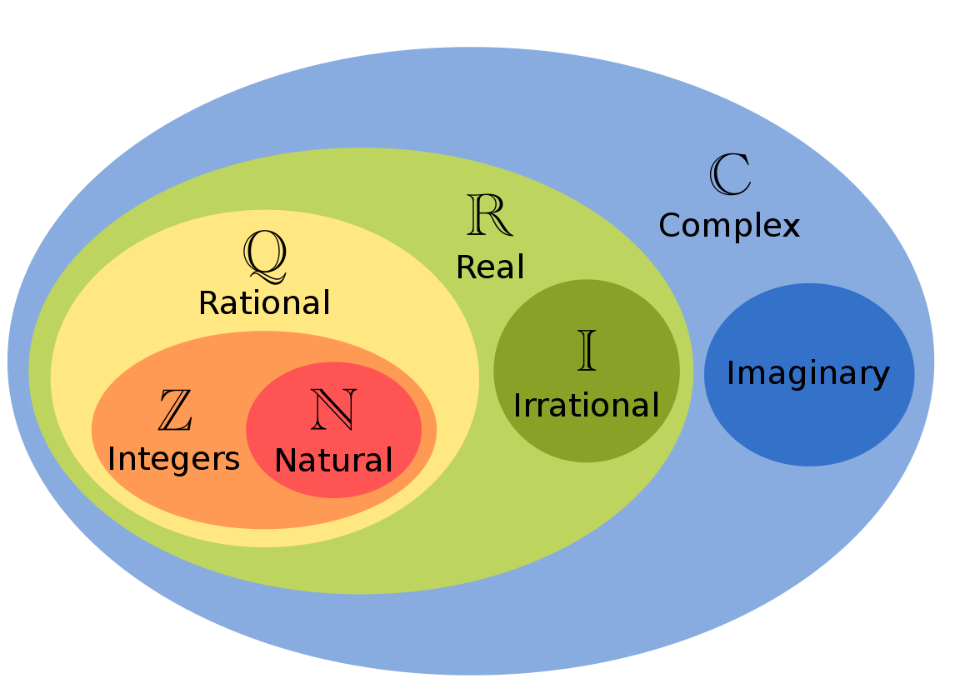
\includegraphics[width=0.5\linewidth]{venn.png}
    \caption{Venn Diagram of Number Sets}
    \label{venn}
\end{figure}

\begin{remark}
    Complex number is currently not a something necessary, as our discussion so far only falls in the real number set.
\end{remark}

\subsection{The Real Number System}
Considering the real numbers are the only system involved so far this book, here, we provide a new mathematical perspective that is different what we were taught, to understand the real number system. We will introduce three axioms that real number holds.
\begin{definition}[Field Axioms]\label{axi:field}
A set \( S \) with operations \( + \) and \( \cdot \) and distinguished elements 0 and 1 with \( 0 \neq 1 \) is a \emph{field} if the following properties hold for all \( x, y, z \in S \):

\begin{itemize}
  \item[A0:] \( x + y \in S \) \hfill Closure
  \item[A1:] \( (x + y) + z = x + (y + z) \) \hfill Associativity
  \item[A2:] \( x + y = y + x \) \hfill Commutativity
  \item[A3:] \( x + 0 = x \) \hfill Identity
  \item[A4:] given \( x \), there is a \( w \in S \) such that \( x + w = 0 \) \hfill Inverse
  \item[M0:] \( x \cdot y \in S \) \hfill Closure
  \item[M1:] \( (x \cdot y) \cdot z = x \cdot (y \cdot z) \) \hfill Associativity
  \item[M2:] \( x \cdot y = y \cdot x \) \hfill Commutativity
  \item[M3:] \( x \cdot 1 = x \) \hfill Identity
  \item[M4:] for \( x \neq 0 \), there is a \( w \in S \) such that \( x \cdot w = 1 \) \hfill Inverse
  \item[DL:] \( x \cdot (y + z) = x \cdot y + x \cdot z \) \hfill Distributive Law
\end{itemize}

\end{definition}
The operations \( + \) and \( \cdot \) are called addition and multiplication. The elements 0 and 1 are the additive identity element and the multiplicative identity element, respectively.   


It follows from these axioms that the additive inverse and multiplicative inverse (of a nonzero \( x \)) are unique. The additive inverse of \( x \) is the \textbf{negative} of \( x \), written as \( -x \). To define subtraction of \( y \) from \( x \), we let \( x - y = x + (-y) \). The multiplicative inverse of \( x \) is the \textbf{reciprocal} of \( x \), written as \( x^{-1} \). \textbf{The element 0 has no reciprocal}. To define division of \( x \) by \( y \) when \( y \neq 0 \), we let \( \frac{x}{y} = x \cdot (y^{-1}) \). We write \( x \cdot y \) as \( xy \) and \( x \cdot x \) as \( x^2 \). We use parentheses where helpful to clarify the order of operations.

\begin{definition}[Order Axioms]\label{axi:order}
     A positive set in a field \( F \) is a set \( P \subset F \) such that for \( x, y \in F \),

\begin{itemize}
  \item[P1:] \( x, y \in P \) implies \( x + y \in P \) \hfill Closure under Addition
  \item[P2:] \( x, y \in P \) implies \( xy \in P \) \hfill Closure under Multiplication
  \item[P3:] \( x \in F \) implies exactly one of \( x = 0 \), \( x \in P \), \( -x \in P \) \hfill Trichotomy
\end{itemize}

An ordered field is a field with a positive set \( P \). In an ordered field, we define \( x < y \) to mean \( y - x \in P \). The relations \( \leq, >, \) and \( \geq \) have analogous definitions in terms of \( P \).

Note that \( P = \{ x \in F : x > 0\} \). Another phrasing of trichotomy is that each ordered pair \( (x, y) \) satisfies exactly one of \( x < y \), \( x = y \), \( x > y \).
If \( S \subseteq F \), then \( \beta \in F \) is an \textbf{upper bound} for \( S \) if \( x \leq \beta \) for all \( x \in S \).
\end{definition}
\begin{definition}[Completeness Theorem]
     An ordered field \( F \) is complete if every nonempty subset of \( F \) that has an upper bound in \( F \) has a least upper bound in \( F \).
\end{definition}

    This theorem ensures the square roots of positive real numbers.

\end{enumerate}

Axiom \autoref{axi:field} and \autoref{axi:order} imply many familiar property of arithmetic:

\begin{proposition}[Arithmetic in $\mathbb{N}$, $\mathbb{Z}$, $\mathbb{Q}$]
Each of $\mathbb{N}$, $\mathbb{Z}$, and $\mathbb{Q}$ is closed under addition and multiplication, $\mathbb{Z}$ and $\mathbb{Q}$ are closed under subtraction, and the set of nonzero numbers in $\mathbb{Q}$ is closed under division.
\end{proposition}

The next four propositions state properties of an ordered field $F$. All statements apply for each choice of $x, y, z, u, v \in F$.

\begin{proposition}
Elementary consequences of the field axioms.
\begin{align*}
    \text{a)} &\quad x + z = y + z \text{ implies } x = y \\
    \text{b)} &\quad x \cdot 0 = 0 \\
    \text{c)} &\quad (-x)y = -(xy) \\
    \text{d)} &\quad -x = (-1)x \\
    \text{e)} &\quad (-x)(-y) = xy \\
    \text{f)} &\quad xz = yz \text{ and } z \neq 0 \text{ imply } x = y \\
    \text{g)} &\quad xy = 0 \text{ implies } x = 0 \text{ or } y = 0
\end{align*}
\end{proposition}

\begin{proposition}[Properties of an ordered field.]
\begin{align*}
    \text{O1:} &\quad x \leq x && \text{Reflexive Property} \\
    \text{O2:} &\quad x < y \text{ and } y < x \text{ imply } x = y && \text{Antisymmetric Property} \\
    \text{O3:} &\quad x < y \text{ and } y < z \text{ imply } x < z && \text{Transitive Property} \\
    \text{O4:} &\quad \text{At least one of } x < y \text{ and } y < x \text{ holds} && \text{Total Ordering Property}
\end{align*}
\end{proposition}

\begin{proposition}[More properties of an ordered field.]
\begin{align*}
    \text{F1:} &\quad x \leq y \text{ implies } x + z \leq y + z && \text{Additive Order Law} \\
    \text{F2:} &\quad x < y \text{ and } 0 < z \text{ imply } xz < yz && \text{Multiplicative Order Law} \\
    \text{F3:} &\quad x < y \text{ and } w < v \text{ imply } x + w < y + v && \text{Addition of Inequalities} \\
    \text{F4:} &\quad 0 \leq x \text{ and } 0 \leq w \text{ imply } xw \leq xw && \text{Multiplication of Inequalities}
\end{align*}
\end{proposition}

\begin{proposition}[Still more properties of an ordered field.]
\begin{align*}
    \text{(a)} &\quad x < y \text{ implies } -y < -x \\
    \text{(b)} &\quad x \leq y \text{ and } z \leq 0 \text{ imply } yz \leq xz \\
    \text{(c)} &\quad 0 \leq x \text{ and } 0 \leq y \text{ imply } 0 \leq xy \\
    \text{(d)} &\quad 0 \leq x^2 \\
    \text{(e)} &\quad 0 < 1 \\
    \text{(f)} &\quad 0 < x \text{ implies } 0 < x^{-1} \\
    \text{(g)} &\quad 0 < x < y \text{ implies } 0 < y^{-1} < x^{-1}
\end{align*}
\end{proposition}




%------------------------------------------------

\chapterimage{orange2.jpg}
\chapterspaceabove{6.75cm} 
\chapterspacebelow{7.25cm} 
\chapter{Inequality}

%------------------------------------------------

\chapterimage{orange2.jpg}
\chapterspaceabove{6.75cm} 
\chapterspacebelow{7.25cm} 
\chapter{Complex Number}

%------------------------------------------------
\part{Further Discrete Mathematics}


\chapterimage{orange2.jpg}
\chapterspaceabove{6.75cm} 
\chapterspacebelow{7.25cm} 
\chapter{Boolean Algebra}

%------------------------------------------------
\chapterimage{orange2.jpg}
\chapterspaceabove{6.75cm} 
\chapterspacebelow{7.25cm} 
\chapter{Preliminary Number Theory}
%------------------------------------------------
\chapterimage{orange2.jpg}
\chapterspaceabove{6.75cm} 
\chapterspacebelow{7.25cm} 
\chapter{Search and Sorting}
%------------------------------------------------
\chapterimage{orange2.jpg}
\chapterspaceabove{6.75cm} 
\chapterspacebelow{7.25cm} 
\chapter{Graph Theory}

%------------------------------------------------
\part{Function and Single-variable Calculus}
%------------------------------------------------
\part{Multi-variable and Vector Calculus}
%------------------------------------------------

\part{Linear Algebra}
%------------------------------------------------
\part{Probability and Combinatorics}

\chapterimage{orange2.jpg}
\chapterspaceabove{6.75cm} 
\chapterspacebelow{7.25cm} 
\chapter{Counting Method and Basic Combinatorics}


\chapterimage{orange2.jpg}
\chapterspaceabove{6.75cm} 
\chapterspacebelow{7.25cm} 
\chapter{Probability Theorems}


\chapterimage{orange2.jpg}
\chapterspaceabove{6.75cm} 
\chapterspacebelow{7.25cm} 
\chapter{Discrete Distribution}


\chapterimage{orange2.jpg}
\chapterspaceabove{6.75cm} 
\chapterspacebelow{7.25cm} 
\chapter{Continuous Distribution}


\chapterimage{orange2.jpg}
\chapterspaceabove{6.75cm} 
\chapterspacebelow{7.25cm} 
\chapter{Joint Cumulative Distribution}
%------------------------------------------------
\part{Statistics}


%----------------------------------------------------------------------------------------

\stopcontents[part] % Manually stop the 'part' table of contents here so the previous Part page table of contents doesn't list the following chapters



\end{document}
